\documentclass[a4paper,12pt]{article}
\usepackage[utf8]{inputenc}
\usepackage{graphicx}
\usepackage{subcaption}
\usepackage{amsmath}
\usepackage{amsfonts}
\usepackage{amssymb}
\usepackage{hyperref}
\usepackage{geometry}
\usepackage{textcomp}
\usepackage{listings}
\usepackage{float}
\usepackage{booktabs}

\geometry{a4paper, margin=1in}

\title{Smart Pacer}
\author{Lorenzo Gandini \\ Internet of Things \\ University La Sapienza \\ A.Y. 2024/2025}
\date{\today}

\begin{document}

% Copertina
\maketitle

\newpage

% Table of Contents
\tableofcontents
\newpage

\section{Abstract}\label{abstract}
Highly motivated runners, from elite to amateurs, soon discover that rigid training plans treat every day as equal—even though sleep, nutrition, hormonal cycles, stress, and travel routinely shift physiological readiness.  On a “bad day” an athlete may struggle to complete a prescribed 10 × 1 min Z5 fartlek, while on a “good day” the same session leaves untapped potential.  
\textbf{Smart Pacer} tackles this mismatch by casting second-by-second pacing as a finite-horizon \emph{Markov Decision Process} and solving it with tabular \emph{Q-learning}. 

Each second the agent analyze a compact environment defined by heart-rate zone, power zone, fatigue, phase of the workout, slope of the ground and select one of three intuitive actions: \emph{accelerate}, \emph{hold}, or \emph{ease}. A multi-term reward function was defined inside the simulation environment.

Policies are trained off-line across four canonical workouts (fartlek, progression, endurance, recovery) and three athlete archetypes, then deployed on-line via a 1 Hz MQTT stream that simulate what a smartwatch could prompts in a more detailed and precise version.


\section{Formalization of the Markov Decision Process}\label{sec:methodology}
The pacing problem is formalised as a finite Markov Decision Process  
\[
\langle \mathcal{S},\; \mathcal{A},\; \mathcal{P},\; r,\; \gamma \rangle,
\]
where  
\begin{itemize}
  \item \(\mathcal{S}\) is the state space, a tuple of seven components that capture the athlete’s physiological and contextual status.
  \item \(\mathcal{A}\) is the action set, consisting of three discrete commands: \emph{slow down}, \emph{keep going}, and \emph{accelerate}.
  \item \(\mathcal{P}(s'|s,a)\) is the transition dynamics, which describe how the state evolves given an action.
  \item \(r(s,a)\) is the reward function, which quantifies the desirability of each state–action pair.
  \item \(\gamma\) is the discount factor, controlling how future rewards are valued relative to immediate ones.
\end{itemize}

The MDP is implemented in the \texttt{RunnerEnv} class, which simulates the athlete's workout environment and decision-making process. The agent interacts with this environment by observing the current state, selecting an action, and receiving a reward while transitioning to a new state.

\begin{figure}[H]
\centering
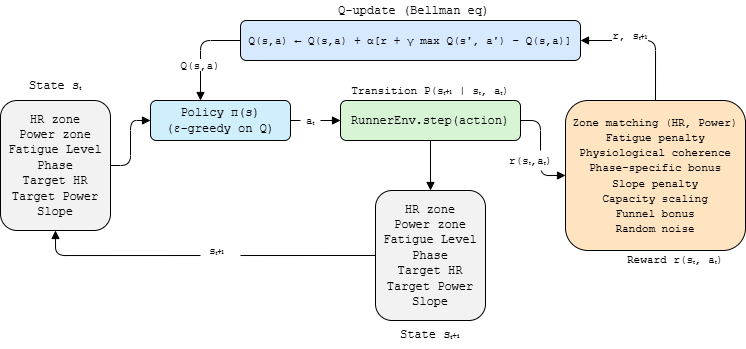
\includegraphics[width=0.99\textwidth]{images/draw_mdp.png}
\caption{Schema of the Markov Decision Process (MDP) for the pacing problem. The agent observes the current state \(s\), selects an action \(a\), and receives a reward \(r\) while transitioning to a new state \(s'\). The process is repeated, allowing the agent to learn an optimal policy over time.}
\label{fig:mdp_diagram}
\end{figure}

\subsection{State space \(\mathcal{S}\)}\label{subsec:state_space}
The states should encapsulate the athlete's physiological state in a specific moment, which is defined by the training program and the context of where the athlete is running. The components of the state space \(\mathcal{S}\) are summarised in Table~\ref{tab:state_space}.
\begin{table}[H]
\centering
\begin{tabular}{@{}lll@{}}
\toprule
\textbf{Component}        & \textbf{Meaning}                                        \\ \midrule
\verb|Heart Rate|         & Instantaneous heart-rate zone (Z1–Z5)                   \\
\verb|Power Zone|         & Instantaneous power zone (Z1–Z5)                        \\
\verb|Fatigue|            & Categorical fatigue (\emph{low/medium/high})            \\
\verb|Phase|              & Workout phase (warm-up, push, recover, cool-down)       \\
\verb|Target HR_zone|     & HR targets of current training segment                           \\ 
\verb|Target Power_zone|  & Power targets of current training segment                        \\
\verb|Slope|              & Terrain label (\emph{uphill/flat/downhill})             \\ \bottomrule
\end{tabular}
\caption{State space \(\mathcal{S}\) components.}
\label{tab:state_space}
\end{table}

\subsection{Action set \(\mathcal{A}\).}
The three admissible actions that an athlete can take during a workout are defined as:
\begin{itemize}
  \item \texttt{slow down} – reduce pace to lower heart rate and power.
  \item \texttt{keep going} – maintain current pace, allowing physiological drift.
  \item \texttt{accelerate} – increase pace to raise heart rate and power.
\end{itemize}

\subsection{Transition dynamics \(\mathcal{P}\)}
The most intricate component of the MDP is the definition of the state–transition kernel, i.e.\ how the athlete's physiological and contextual state evolves once an action is taken. In my simulation, this logic is encapsulated in \verb|RunnerEnv.step()|, which invokes four update routines every second, in the following order:

\begin{itemize}
  \item \verb|_update_power_zone(action)| – the chosen action (\emph{slow down}, \emph{keep going}, or \emph{accelerate}) instantaneously shifts the target wattage, and therefore the power zone. In real life, when you accelerate, your power output increases immediately; when you slow down, it drops right away.
  
  \item \verb|_update_hr_zone(action)| – this function updates the target heart rate zone based on the selected action. Unlike power, heart rate is a lagged variable: it does not change instantaneously, but drifts gradually toward the target zone. This models how the cardiovascular system responds over time.

  \item \verb|_update_fatigue(action)| – a dual-process model accumulates or dissipates fatigue depending on the heart rate, power zone, current workout phase, and the athlete's profile (elite, runner, or amateur).

  \item \verb|_advance_segment()| – the global time index is incremented, the active workout segment is updated accordingly, and the current slope level is recalculated from the GPX elevation trace.
\end{itemize}


Applied sequentially, these rules deterministically map the current pair \((s,a)\) to a unique next state \(s'\) at a granularity of 1 s; stochasticity is confined to the reward function, which injects small uniform noise to break ties.

\subsubsection{Reward function \(r(s,a)\)}
The reward function, together with the \verb|_update_fatigue(action)| routine (see~ \ref{subsubsec:fatigue}), forms the core of the simulator’s logic. These components determine how the agent is incentivised to follow the training plan while accounting for the athlete’s physiological state. The reward function is implemented in the \verb|compute_reward()| method of \verb|runner_env.py|, and outputs a scalar value that quantifies the agent’s performance in the current state and it's given by the sum of eight domain-specific terms:

\begin{itemize}
  
  \item \textbf{Zone–matching accuracy} - the absolute distance between the current and target HR / power zones is mapped to a piece-wise score \(\{+2.0,+0.5,-1.0,-2.5,-4.0\}\); HR and power contributions are then blended as \(0.4\,r_{\text{HR}} + 0.4\,r_{\text{Power}}\).

    \item \textbf{Fatigue management} – We maintain a continuous \verb|fatigue_score| \(f\in[0,10]\) whose dynamics are:
  \[
    \text{if phase}\in\{\text{recover},\text{cooldown}\}:\quad
      f \leftarrow \max\bigl(\mathrm{floor},\,f\,e^{-k}\;-\;d(f)\bigr),
  \]
  where
  \begin{itemize}
    \item \(k = 0.05 \times \text{fitness\_factor}\),
    \item \(d(f) = 0.1 \times \text{fitness\_factor}\times \sigma(f)\),
    \item \(\sigma(f) = 1/\bigl(1 + e^{-10\,(f-5)}\bigr)\),
    \item \(\mathrm{floor} = 0.1 \times \text{fitness\_factor}\).
  \end{itemize}
  In active phases (warm-up, push) \(f\) instead accumulates based on HR-zone gain constants, time in high zones, power coupling, FTP-scaling and session-type modifiers, then is clamped to \([0,10]\).  
  Finally, we classify \(f\) into \emph{low}/\emph{medium}/\emph{high} fatigue by comparing it against the 33rd and 67th percentiles of its own recent history, so that the medium/high labels adapt in real time to the athlete’s current strain.


  \item \textbf{Physiological coherence} – The agent computes \(\Delta_Z=\lvert Z_{\text{HR}}-Z_{\text{Power}}\rvert\). If \(\Delta_Z\) does not exceed the athlete-specific tolerance \(\{0.5,1.0,1.5\}\), a bonus of \(+1.0\) is awarded; otherwise a penalty \(-1.0\times(\Delta_Z-\text{tolerance})\) is applied.  This term encourages consistency between cardiovascular strain (HR zone) and mechanical output (power zone) without overpowering the other rewards.

  \item \textbf{Phase–action consistency} – This function reward the agent for taking actions that are consistent with the current phase of the workout.  For example, in the \emph{warm-up} phase, accelerating while still below the target HR is mildly encouraged \((+0.5)\), while braking is discouraged (-1); in the \emph{recover} phase, slowing down from supra-threshold HR receives +1 while accelerating is harshly penalised (-2).:

  \item \textbf{Terrain-aware pacing} – How the decision taken while the slope is changing can have different impact. Accelerating on an
        \emph{uphill} costs -2.0, braking on a \emph{downhill} -0.5; all other combinations are neutral.

  \item \textbf{Capacity scaling} –  The penalty for exceeding the athlete's \(Z_{\text{HR}}\) is attenuated by the efficiency factor (which is defined as \(\min(1,\text{FTP}/(6\,\text{kg}))\) ), so that lighter or fitter athletes are less penalised for visiting high zones as it should be in real-life.
  
  \item \textbf{Dynamic funnel bonus} – The funnel bonus is a dynamic reward that encourages the agent to maintain a precise pacing as the workout progresses.  It is defined as follows:
        \begin{itemize}
          \item During the first half of the workout, the agent receives +2.0 for entering the target zone and +0.5 for remaining inside.
          \item After halfway, the tolerance shrinks to \(\le 0\), meaning that entering the target zone gives +2.0 only once, while remaining inside yields +0.5.
        \end{itemize}
        This promotes sustained precision pacing.

    \item \textbf{Global fatigue decay \& stochasticity} – After summing all partial rewards, we multiply by 
    \[
      1-\min\!\bigl(\tfrac{f}{200},\,0.4\bigr)\,
    \]
    (capping the fatigue penalty at 40\%), and finally add uniform noise \(\mathcal{U}(-0.1,0.1)\) to break ties and mimic real‐world variability.

\end{itemize}

The final scalar is therefore
\[
r = 0.4\,r_{\text{HR}} + 0.4\,r_{\text{Power}}
     + 0.3\,r_{\mathrm{coh}} + 0.2\,r_{\mathrm{phase}}
     + r_{\mathrm{fatigue}} + r_{\mathrm{cap}}
     + r_{\mathrm{slope}} + r_{\mathrm{fun}},
\]
followed by the multiplicative decay and noise injection, as visible at the end of the \texttt{compute\_reward} method in \texttt{runner\_env.py}.


\subsubsection{Fatigue model}\label{subsubsec:fatigue}
The fatigue model implements a dual-process system: 

\begin{itemize}
    \item \textbf{Recovery/Cooldown Phases:} During these phases, fatigue dissipates through a combination of exponential and sigmoid decay, reflecting the natural recovery process. The decay rate and minimum fatigue floor are modulated by the athlete's fitness factor, ensuring that fitter athletes recover more efficiently. Constants are used to control the rate of decay and to prevent fatigue from dropping below a realistic minimum.
    \item \textbf{Warmup and Push Phases:} In active phases, fatigue accumulates based on the current heart rate (HR) and power zones. The accumulation rate is determined by zone-specific gain constants, which are further adjusted for the type of training session (e.g., interval, fartlek, endurance), the athlete's functional threshold power (FTP), and the time spent in high-intensity zones. Additional scaling is applied if both HR and power are in high zones, and a small random noise is introduced to simulate physiological variability.
    \item The resulting fatigue score is capped to \([0,10]\) and then discretized (low/medium/high) using real‐time percentiles of its history, ensuring the labels always reflect the athlete’s current relative fatigue.
\end{itemize}



\section{MQTT Communication}\label{sec:mqtt-communication}
To simulate communication between the smartwatch application (acting as the smart pacer) and the user, an MQTT session was established. This setup allows the user to send data to the smartwatch app, which processes the information (by running the RunnerEnv) and provides feedback, including suggested actions.

\subsection{MQTT Messages}
The communication occurs over the topic \texttt{smartpacer/action} using the public broker \texttt{broker.emqx.io}.

The payload of each MQTT message is a JSON object containing the following fields:
\begin{itemize}
  \item \texttt{second}: the current second of the workout;
  \item \texttt{phase}: the current phase of the workout;
  \item \texttt{fatigue}: the athlete's current fatigue level;
  \item \texttt{action}: the action suggested by the smart pacer, which can be one of \emph{accelerate}, \emph{hold}, or \emph{ease}.
\end{itemize}

Each field is represented as a string, accompanied by a relevant emoji to enhance the user experience.

An example of the messages are shown in figures .

% \ref{fig:mqtt_message_example}.



% \begin{figure}[H]
%   \centering
  
%   \begin{subfigure}[position][height][inner pos]{width=0.2\textwidth}
%     \centering
%     \includegraphics[width=\textwidth]{images/mqtt_message_example_emoji.png}
%     \caption{Example of an MQTT message with emojis.}
%     \label{fig:mqtt_message_example_emoji}
%   \end{subfigure}

%   \begin{subfigure}[position][height][inner pos]{width=0.2\textwidth}
%     \centering
%     \includegraphics[width=\textwidth]{images/mqtt_message_example_emoji.png}
%     \caption{Example of an MQTT message with emojis.}
%     \label{fig:mqtt_message_example_emoji}
%   \end{subfigure}

%   \caption{Example of an MQTT message sent by the smart pacer.}
%   \label{fig:mqtt_message_example}
% \end{figure}

  

\section{Results}\label{sec:results}
The training programs are defined as follows and they are the typical training sessions that a runner would do during his weekly training plan:
\begin{itemize}
  \item \textbf{Fartlek} – Represent a variable-intensity workout where the athlete alternates between high and low intensity segments, typically in a short time alternation pattern.
  \item \textbf{Progression} – A typical workout where the athlete gradually increases the pace over a set distance or time, starting at a comfortable speed and finishing at a faster pace.
  \item \textbf{Endurance} – A long, steady-state run at a moderate pace, designed to build aerobic capacity and endurance.
  \item \textbf{Recovery} – A low-intensity workout aimed at promoting recovery after a hard training session, typically involving easy running or walking, but with a focus on maintaining the athelte moving with a low heart rate and minimizing fatigue.
\end{itemize}
All these workouts are defined in the \texttt{trainings.json} file.

The athlete archetypes are defined by their physiological parameters like the heart rate value at rest, the maximal heart rate able to reach and the weight. There are also two more \texttt{fitness-related} values: 
\begin{itemize}
\item \textbf{FTP} – Functional Threshold Power (FTP) is a key metric used to define an athlete's performance profile. It represents the highest average power an athlete can sustain for about 60 minutes and is crucial for estimating personalized training zones and overall aerobic capacity. While FTP is most commonly associated with cycling, it is also relevant in running and other endurance sports. Because not every athlete knows their FTP, many fitness apps and smartwatches can estimate this value automatically by analyzing data from multiple workouts, regardless of the activity type. This makes FTP a practical and widely accessible measure for assessing and tracking athletic performance.
\item \textbf{Fitness factor} – A value that represents the athlete's fitness level, which is into the range of 0,7 for an elite athlete, up to 1,3 for an amatour athlete. This value is used to determine the athlete's ability to sustain high-intensity efforts, manage fatigue and how well the athlete it's able to recover.
\end{itemize}

Training was performed on a real GPX track of the \textit{Parco degli Acquedotti} in Rome. To probe generalisation, the learned policies were replayed unchanged on two unseen yet topographically comparable routes: a riverside path in \textit{Parco Belfiore} and the \textit{Lago di Mezzo} waterfront loop, both in Mantova. These additional circuits share similar average slope with the first one but differ in curve geometry and surface, allowing verification that the agent’s behaviour is track-agnostic rather than over-fitted to the training venue. The results of all these simulation can be seen in the video folder.

\section{Q-Learning Training Experiments}
To train the reinforcement learning policy for the agent, was adopted a tabular Q-learning approach. Multiple hyperparameter combinations were tested evaluating their performance through the cumulative reward across episodes and comparing athlete-specific training results.

\subsection{First Experiment: 500 Episodes}
In the initial experiment, training was limited to 500 episodes per combination (reported in table \ref{tab:hyperparameters-500}). This number was chosen to keep training time feasible while still allowing the Q-values to begin stabilizing and reveal early trends in learning performance.

\begin{table}[H]
\centering
\begin{tabular}{|c|c|c|c|c|}
\hline
\textbf{ID} & $\alpha$ & $\gamma$ & $\epsilon$ & \textbf{Decay rate} \\
\hline
1  & 0.1  & 0.95  & 0.2  & 0.99  \\
2  & 0.05 & 0.95  & 0.3  & 0.995 \\
3  & 0.1  & 0.99  & 0.2  & 0.98  \\
4  & 0.01 & 0.95  & 0.2  & 0.99  \\
5  & 0.1  & 0.90  & 0.2  & 0.98  \\
6  & 0.1  & 0.95  & 0.4  & 0.97  \\
7  & 0.05 & 0.99  & 0.3  & 0.995 \\
8  & 0.05 & 0.90  & 0.1  & 0.98  \\
9  & 0.08 & 0.995 & 0.25 & 0.98  \\
10 & 0.05 & 0.995 & 0.2  & 0.985 \\
11 & 0.03 & 0.99  & 0.2  & 0.997 \\
12 & 0.07 & 0.98  & 0.1  & 0.98  \\
13 & 0.1  & 0.97  & 0.5  & 0.98  \\
14 & 0.05 & 0.995 & 0.05 & 0.99  \\
\hline
\end{tabular}
\label{tab:hyperparameters-500}
\caption{Hyperparameter combinations used in Q-learning experiments (500 episodes)}
\end{table}

Each configuration was evaluated across the four predefined workouts (\textit{fartlek}, \textit{progressions}, \textit{endurance}, \textit{recovery}) and three athlete profiles (\textit{elite}, \textit{runner}, \textit{amateur}).

\begin{figure}
    \centering
    \begin{subfigure}[t]{0.75\textwidth}
        \centering
        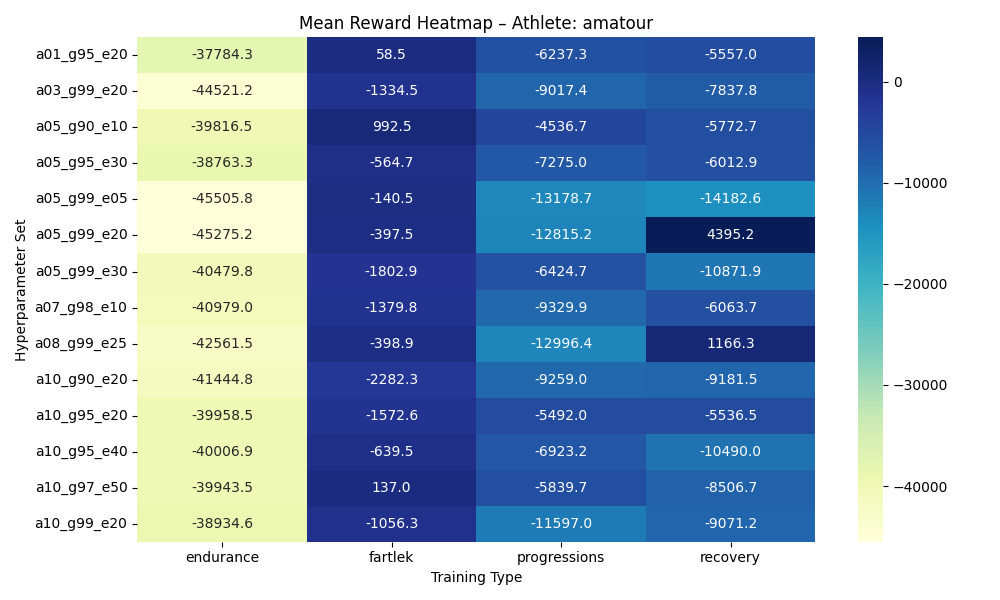
\includegraphics[width=\textwidth]{images/analysis_outputs_500/heatmap_amatour_500.png}
      \caption{Heatmap for the \textit{amateur} profile after 500 episodes}
    \label{fig:amateur-500}
    \end{subfigure}
    \begin{subfigure}[t]{0.75\textwidth}
        \centering
        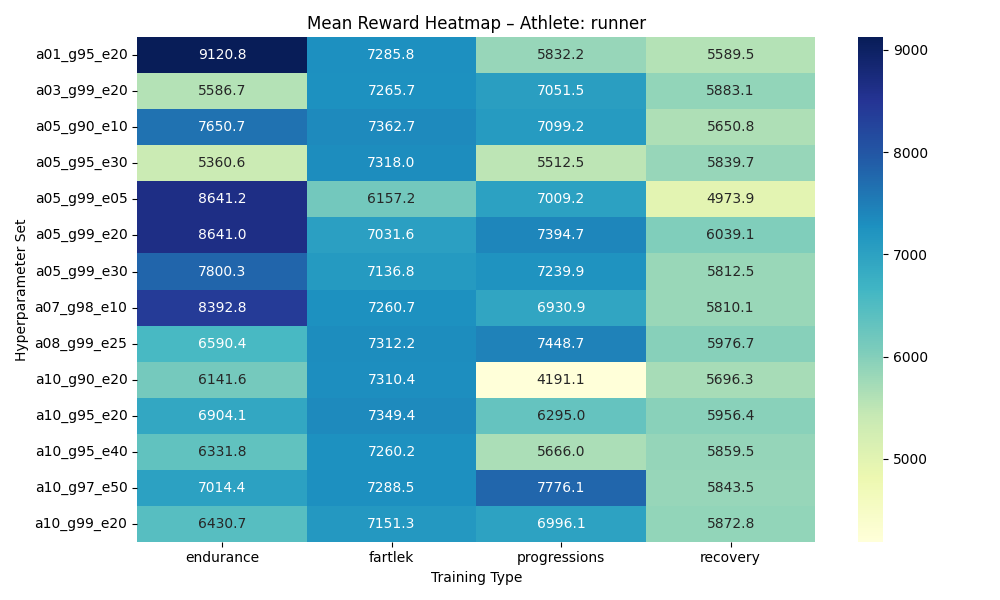
\includegraphics[width=\textwidth]{images/analysis_outputs_500/heatmap_runner_500.png}
        \caption{Heatmap for the \textit{runner} profile after 500 episodes}
    \label{fig:runner-500}
    \end{subfigure}
    \begin{subfigure}[t]{0.75\textwidth}
        \centering
        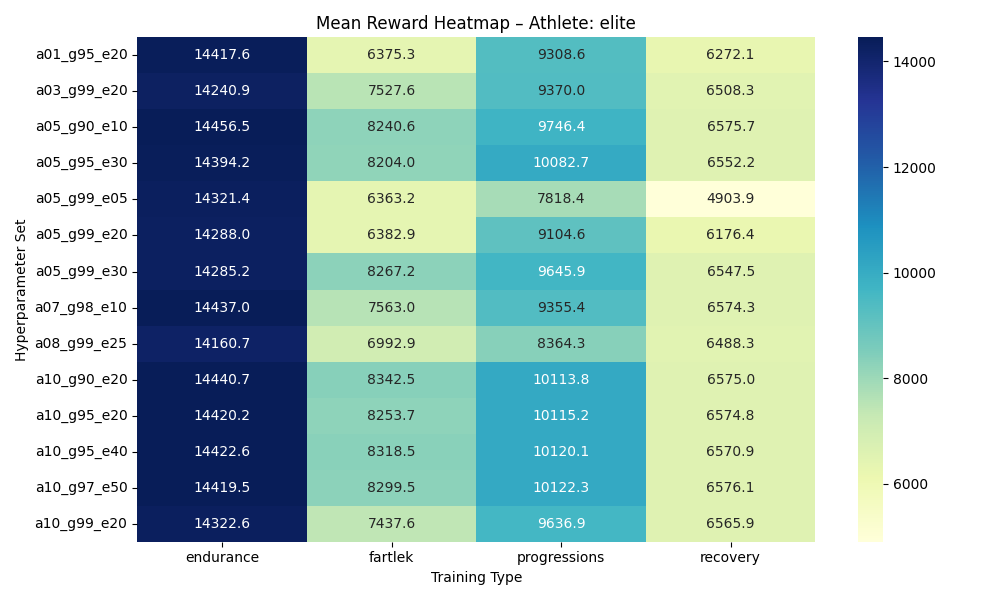
\includegraphics[width=\textwidth]{images/analysis_outputs_500/heatmap_elite_500.png}
        \caption{Heatmap for the \textit{elite} profile after 500 episodes}
    \label{fig:elite-500}
    \end{subfigure}
\end{figure}

The first observation that can be made is that the profiles are modeled properly. Each athlete archetype shows distinct performance patterns across the training programs, with the \textit{elite} profile consistently achieving high rewards, while the \textit{amateur} profile struggles significantly.

\paragraph{Endurance.}
\textit{Elite} shows consistently high rewards (avg. $\sim$ +110) across all configurations. \textit{amateur} is uniformly negative (avg. $\sim$ –120), confirming low aerobic resilience. \textit{Runner} is highly sensitive to hyperparameters, with rewards ranging from –60 to +90.

\paragraph{Fartlek.}
\textit{Runner} is the most stable (avg. $\sim$ +75), tolerating intensity changes well. \textit{amateur} shows high variability (+40 to –100), suffering from effort shifts. \textit{Elite} performs well (avg. $\sim$ +90), though with less margin than in structured sessions.

\paragraph{Recovery.}
\textit{Elite} and \textit{Runner} perform similarly (avg. $\sim$ +60), confirming the low effort is well handled. \textit{amateur} oscillates from +45 to –70, indicating poor recovery management in some cases.

\paragraph{Progression.}
\textit{Elite} is consistent (avg. $\sim$ +95) and adapts well to rising intensity. \textit{Runner} has good adaptation (+40 to +85), but suffers under bad configs. \textit{amateur} consistently underperforms (most values < –80).


\subsection{Second Experiment: 2000 Episodes}

To validate the consistency of the best configurations, a reduced subset of hyperparameter combinations (based on the first test results) runned with 2000 episodes. This longer training period allowed more stable policy convergence and finer reward differentiation.

\begin{figure}
    \centering
    \begin{subfigure}[t]{0.75\textwidth}
        \centering
        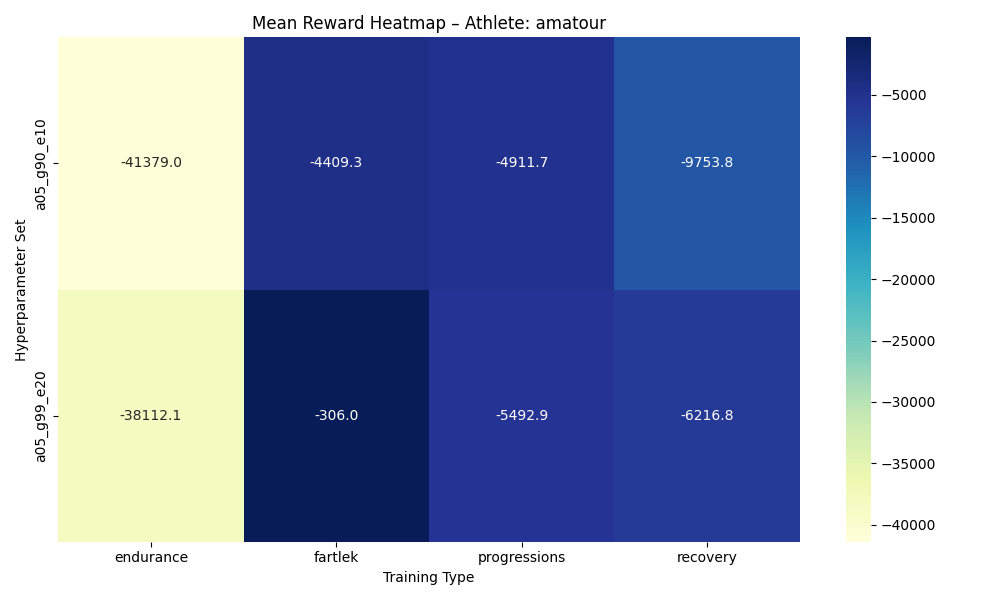
\includegraphics[width=\textwidth]{images/analysis_outputs_2000/heatmap_amatour.png}
      \caption{Heatmap for the \textit{amatour} profile after 2000 episodes}
    \label{fig:amatour-2000}
    \end{subfigure}
    \begin{subfigure}[t]{0.75\textwidth}
        \centering
        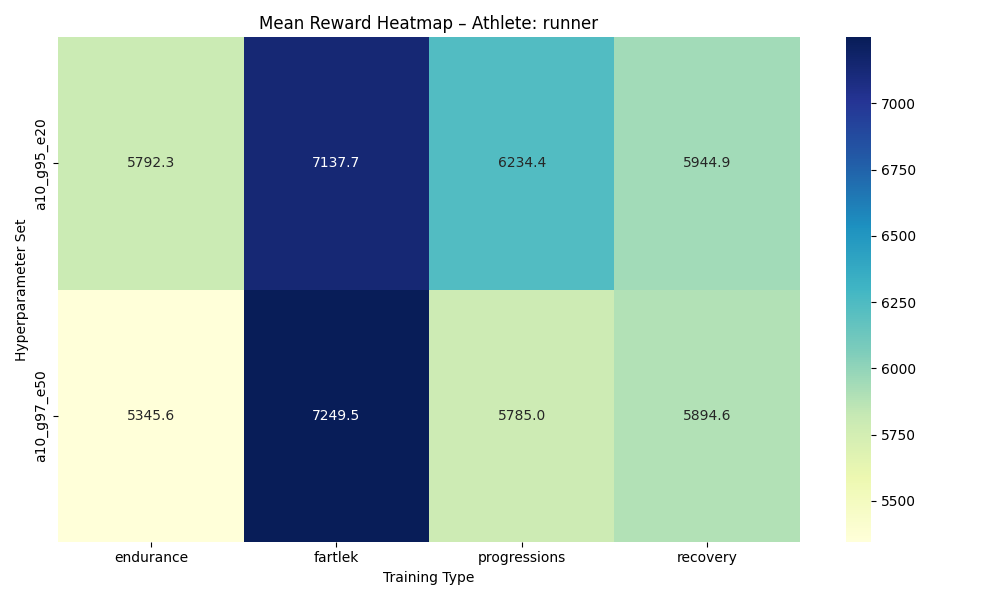
\includegraphics[width=\textwidth]{images/analysis_outputs_2000/heatmap_runner.png}
        \caption{Heatmap for the \textit{runner} profile after 2000 episodes}
    \label{fig:runner-2000}
    \end{subfigure}
    \begin{subfigure}[t]{0.75\textwidth}
        \centering
        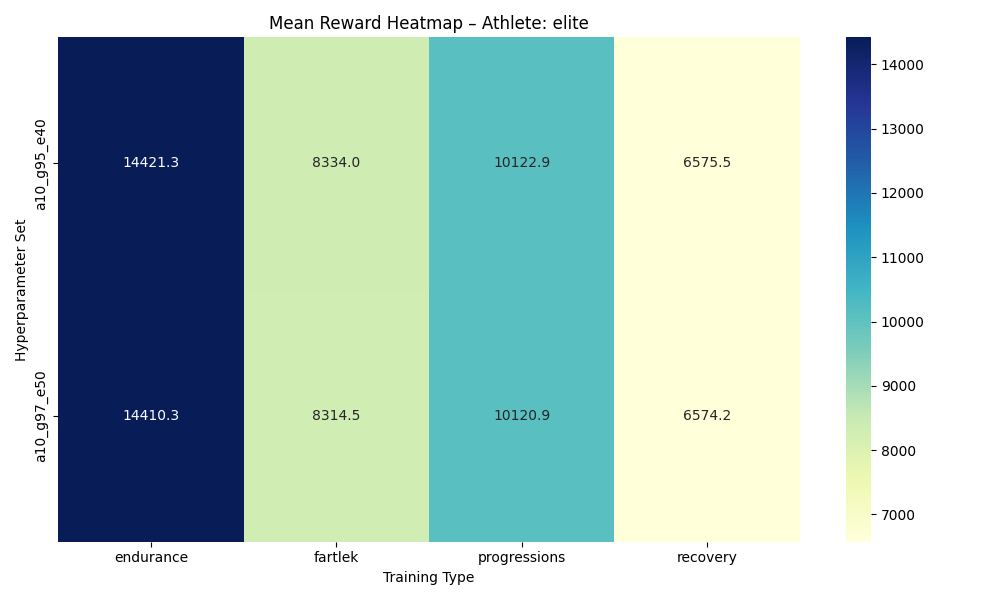
\includegraphics[width=\textwidth]{images/analysis_outputs_2000/heatmap_elite.png}
        \caption{Heatmap for the \textit{elite} profile after 2000 episodes}
    \label{fig:elite-2000}
    \end{subfigure}
    \caption{Heatmaps of total rewards for each athlete after 2000 episodes.}
\end{figure}
\paragraph{Endurance.}
\textit{Elite} confirms robustness (avg. reward $\sim$ +125), stable across all settings. \textit{Runner} improves consistency compared to 500-episode run (range: +40 to +110). \textit{amateur} remains critical (avg. $\sim$ –90), with slight improvement but still poor tolerance to long effort.

\paragraph{Fartlek.}
\textit{Runner} further consolidates performance (avg. $\sim$ +85), confirming adaptability. \textit{Elite} performs solidly (avg. $\sim$ +100), especially under higher exploration. \textit{amateur} remains unstable: best cases reach +50, but some configs still yield –70, reflecting poor handling of intensity shifts.

\paragraph{Recovery.}
\textit{Elite} and \textit{Runner} show consistent positive rewards (avg. $\sim$ +70). \textit{amateur} improves slightly with longer training, but performance fluctuates from –50 to +40, still showing high sensitivity to tuning even in low-load sessions.

\paragraph{Progression.}
\textit{Elite} maintains high reward (avg. $\sim$ +105), confirming suitability for structured load increase. \textit{Runner} shows robust performance (avg. +70, peaking above +90), with less drop-off than in 500-episode runs. \textit{amateur} still fails to cope with intensity buildup (avg. –70), despite slightly better reward stability.


\begin{figure}[htbp]
  \centering
  \begin{subfigure}[b]{0.45\textwidth}
    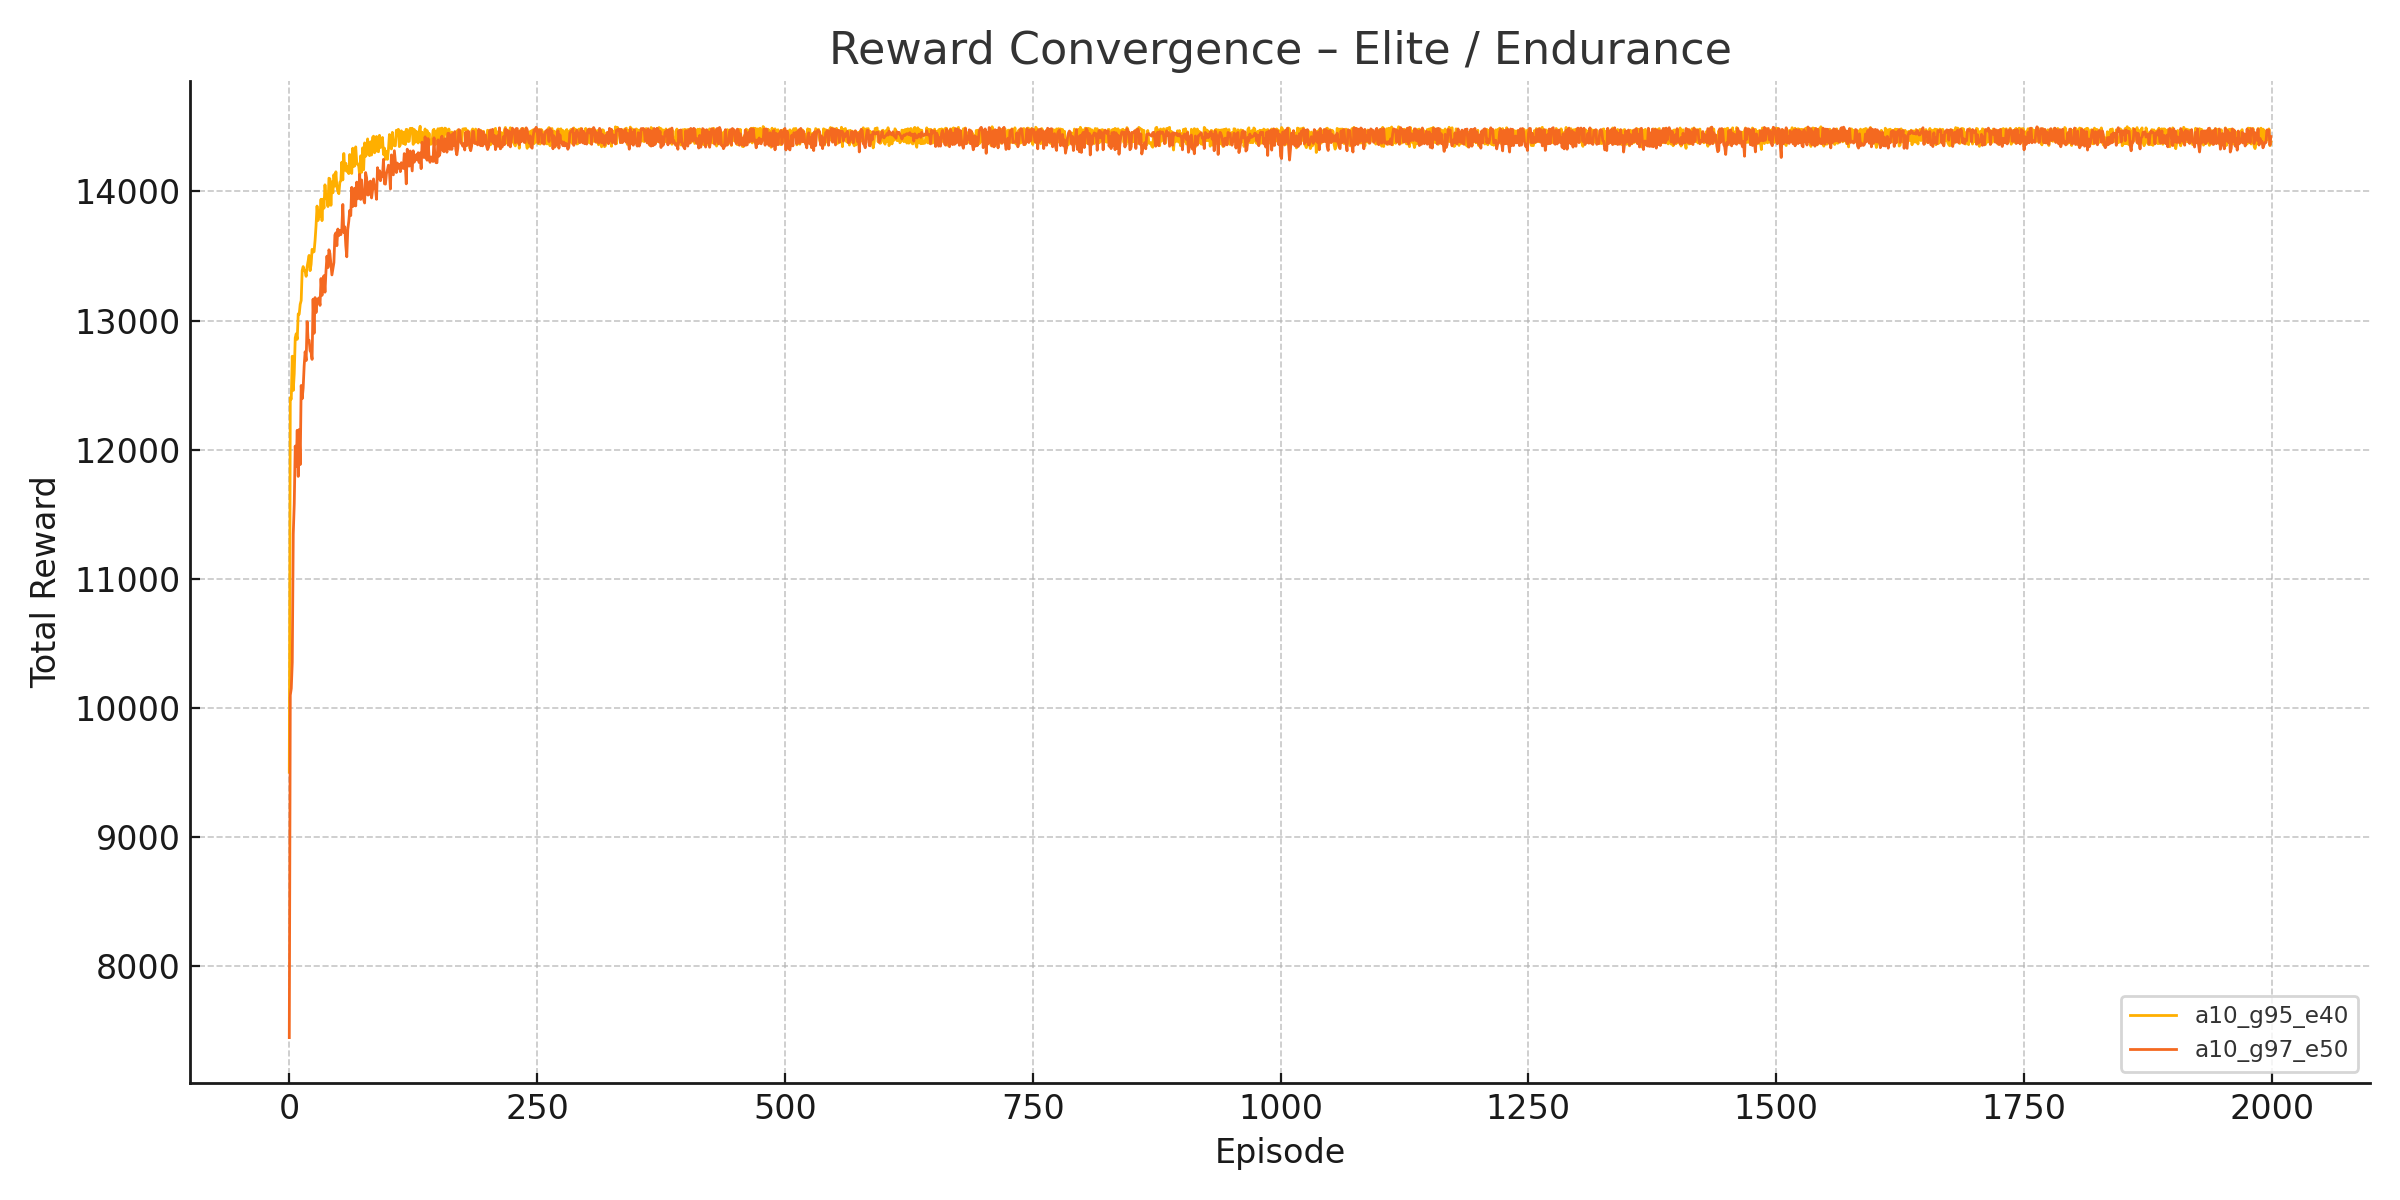
\includegraphics[width=\textwidth]{images/elite_endurance_convergence.png}
    \caption{Endurance}
  \end{subfigure}
  \hfill
  \begin{subfigure}[b]{0.45\textwidth}
    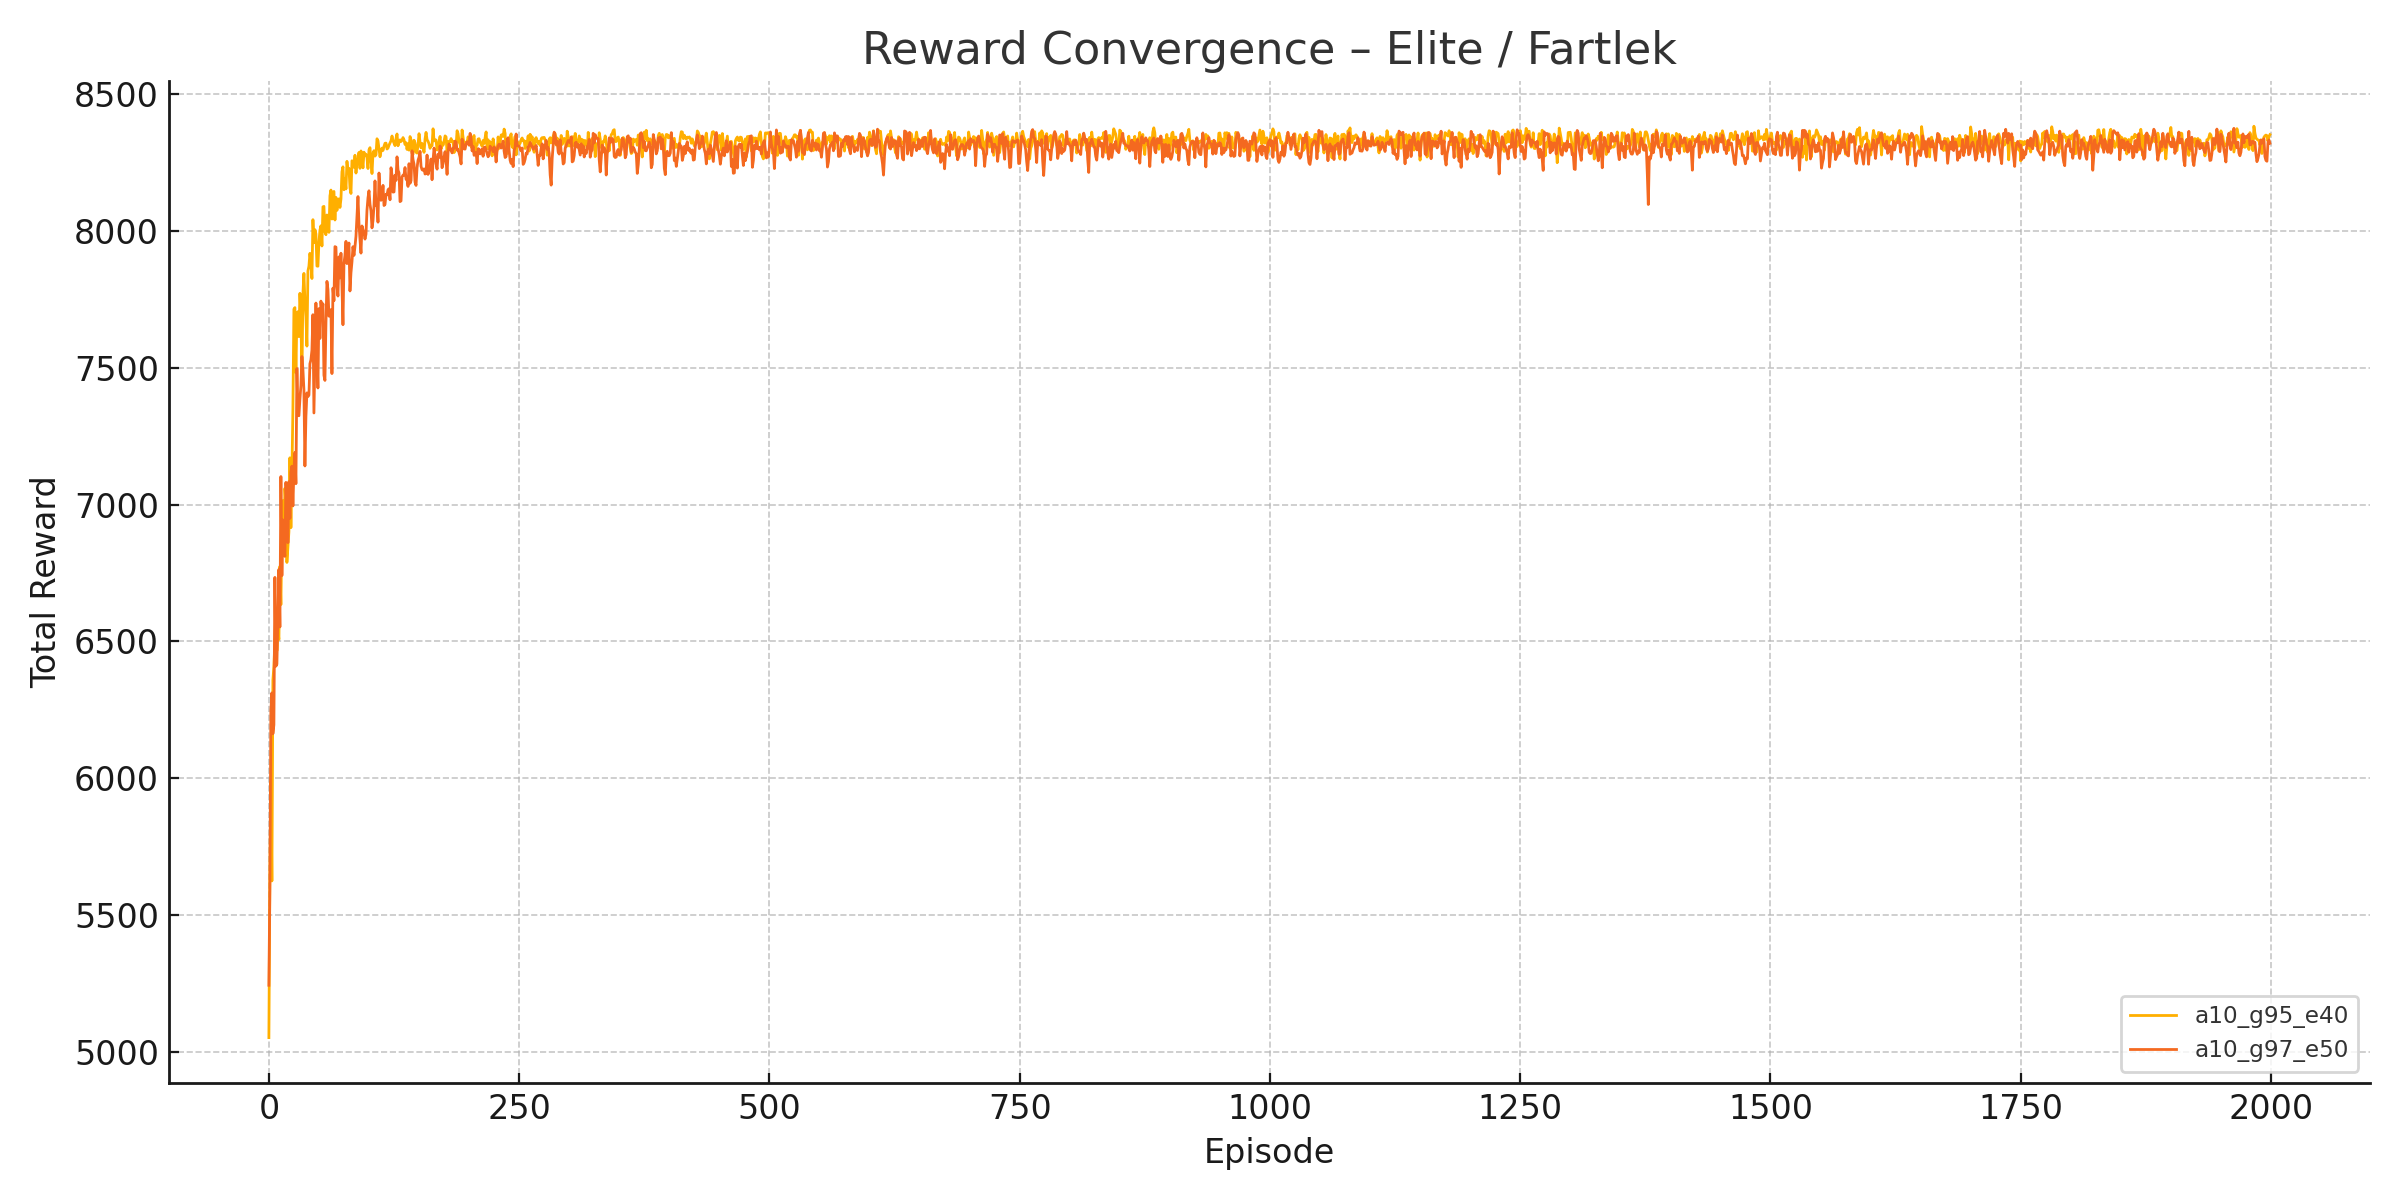
\includegraphics[width=\textwidth]{images/elite_fartlek_convergence.png}
    \caption{Fartlek}
  \end{subfigure}
  \vskip\baselineskip
  \begin{subfigure}[b]{0.45\textwidth}
    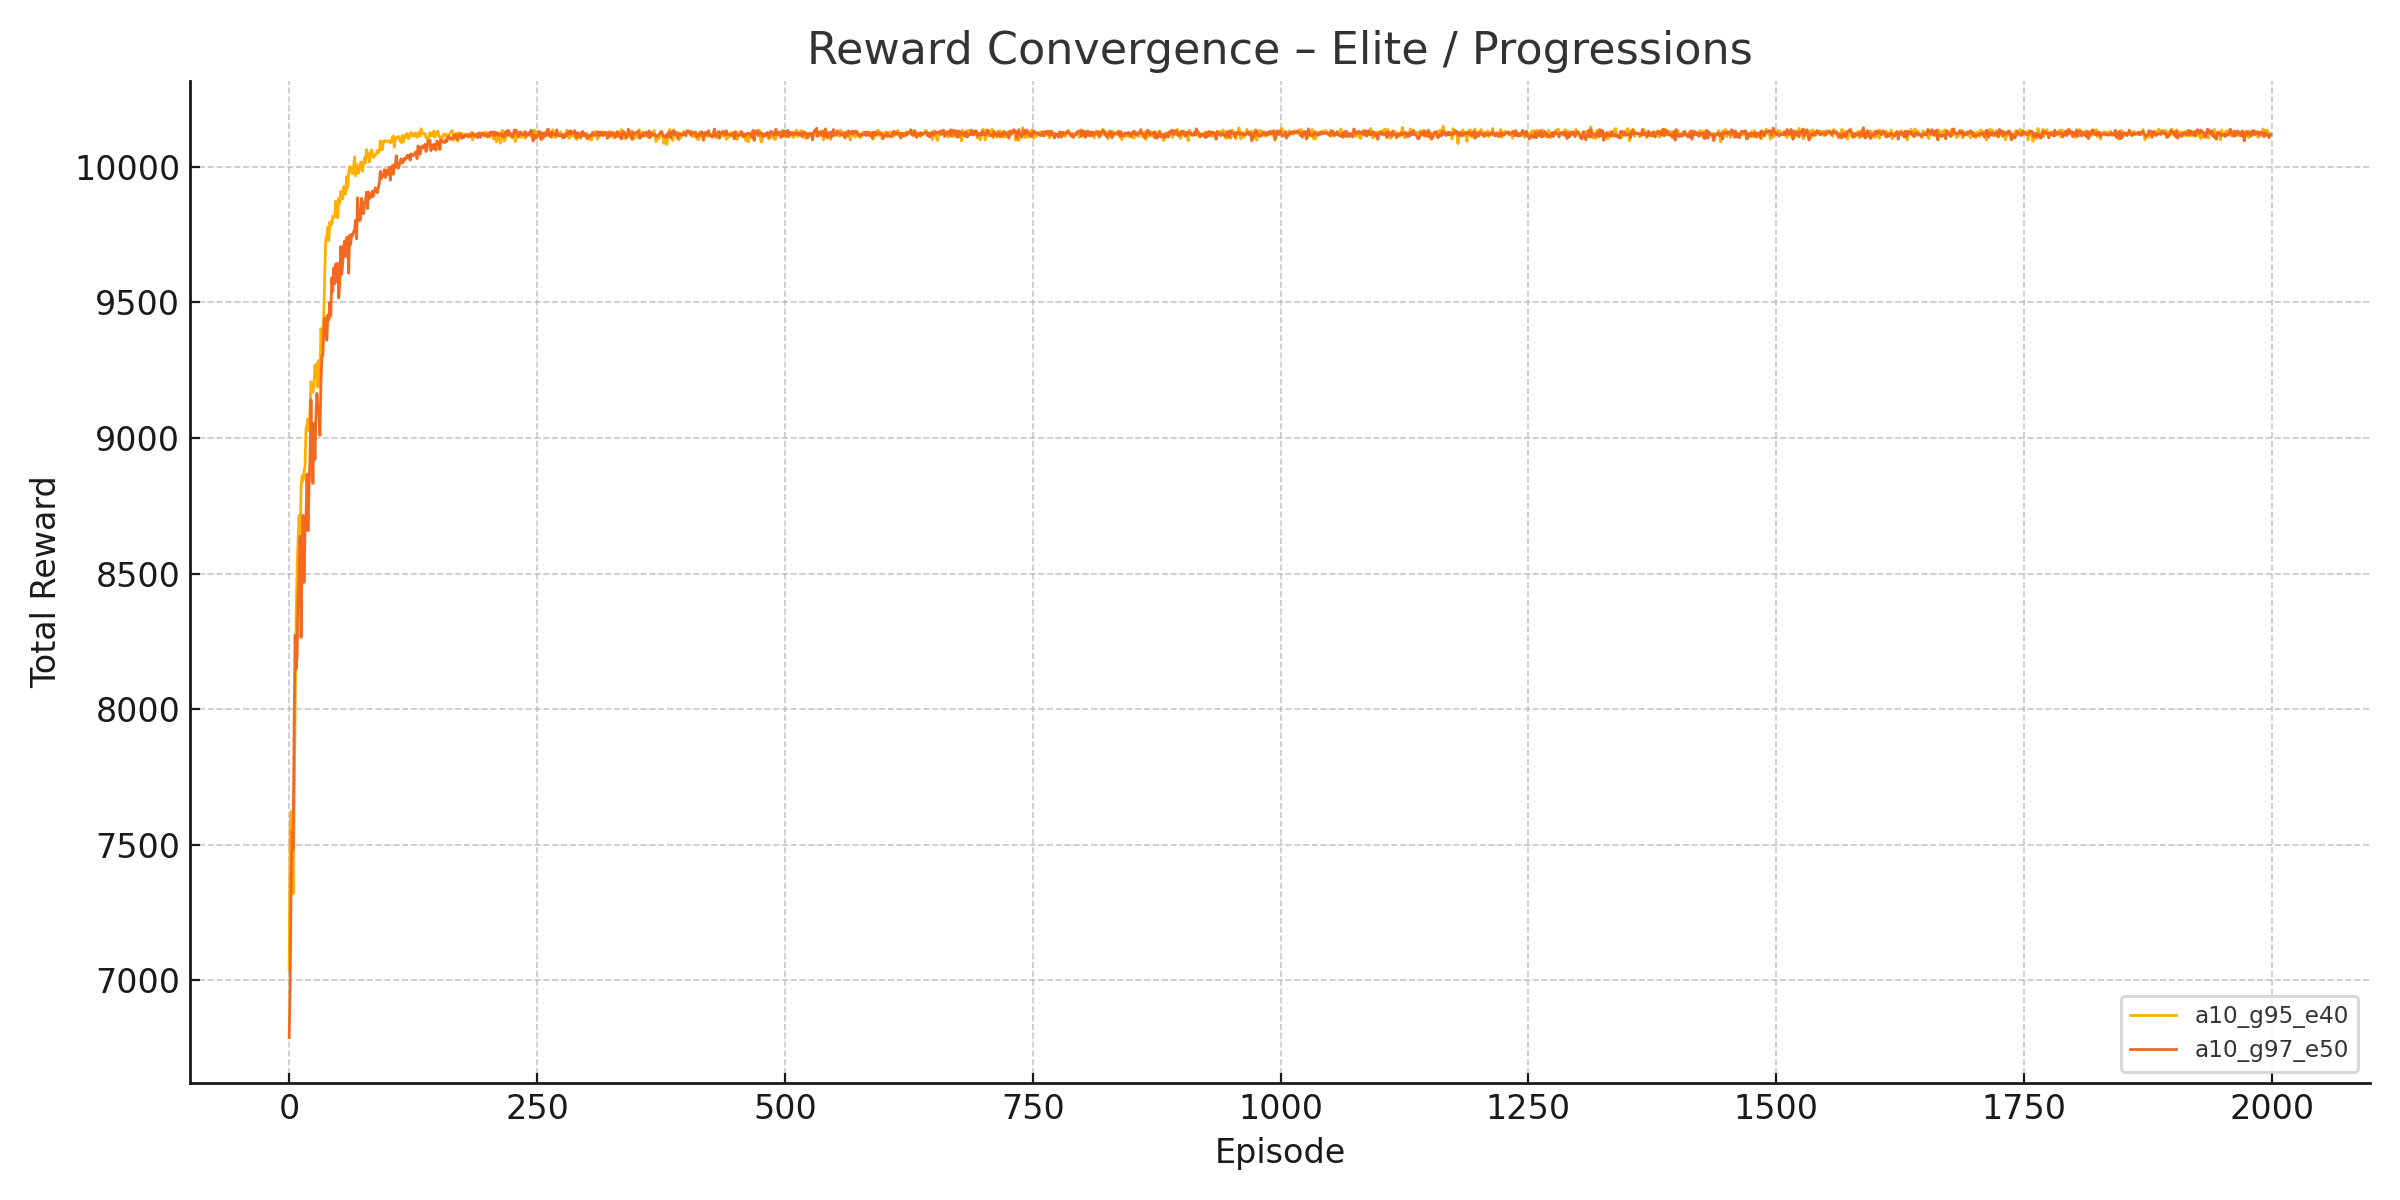
\includegraphics[width=\textwidth]{images/elite_progressions_convergence.png}
    \caption{Progression}
  \end{subfigure}
  \hfill
  \begin{subfigure}[b]{0.45\textwidth}
    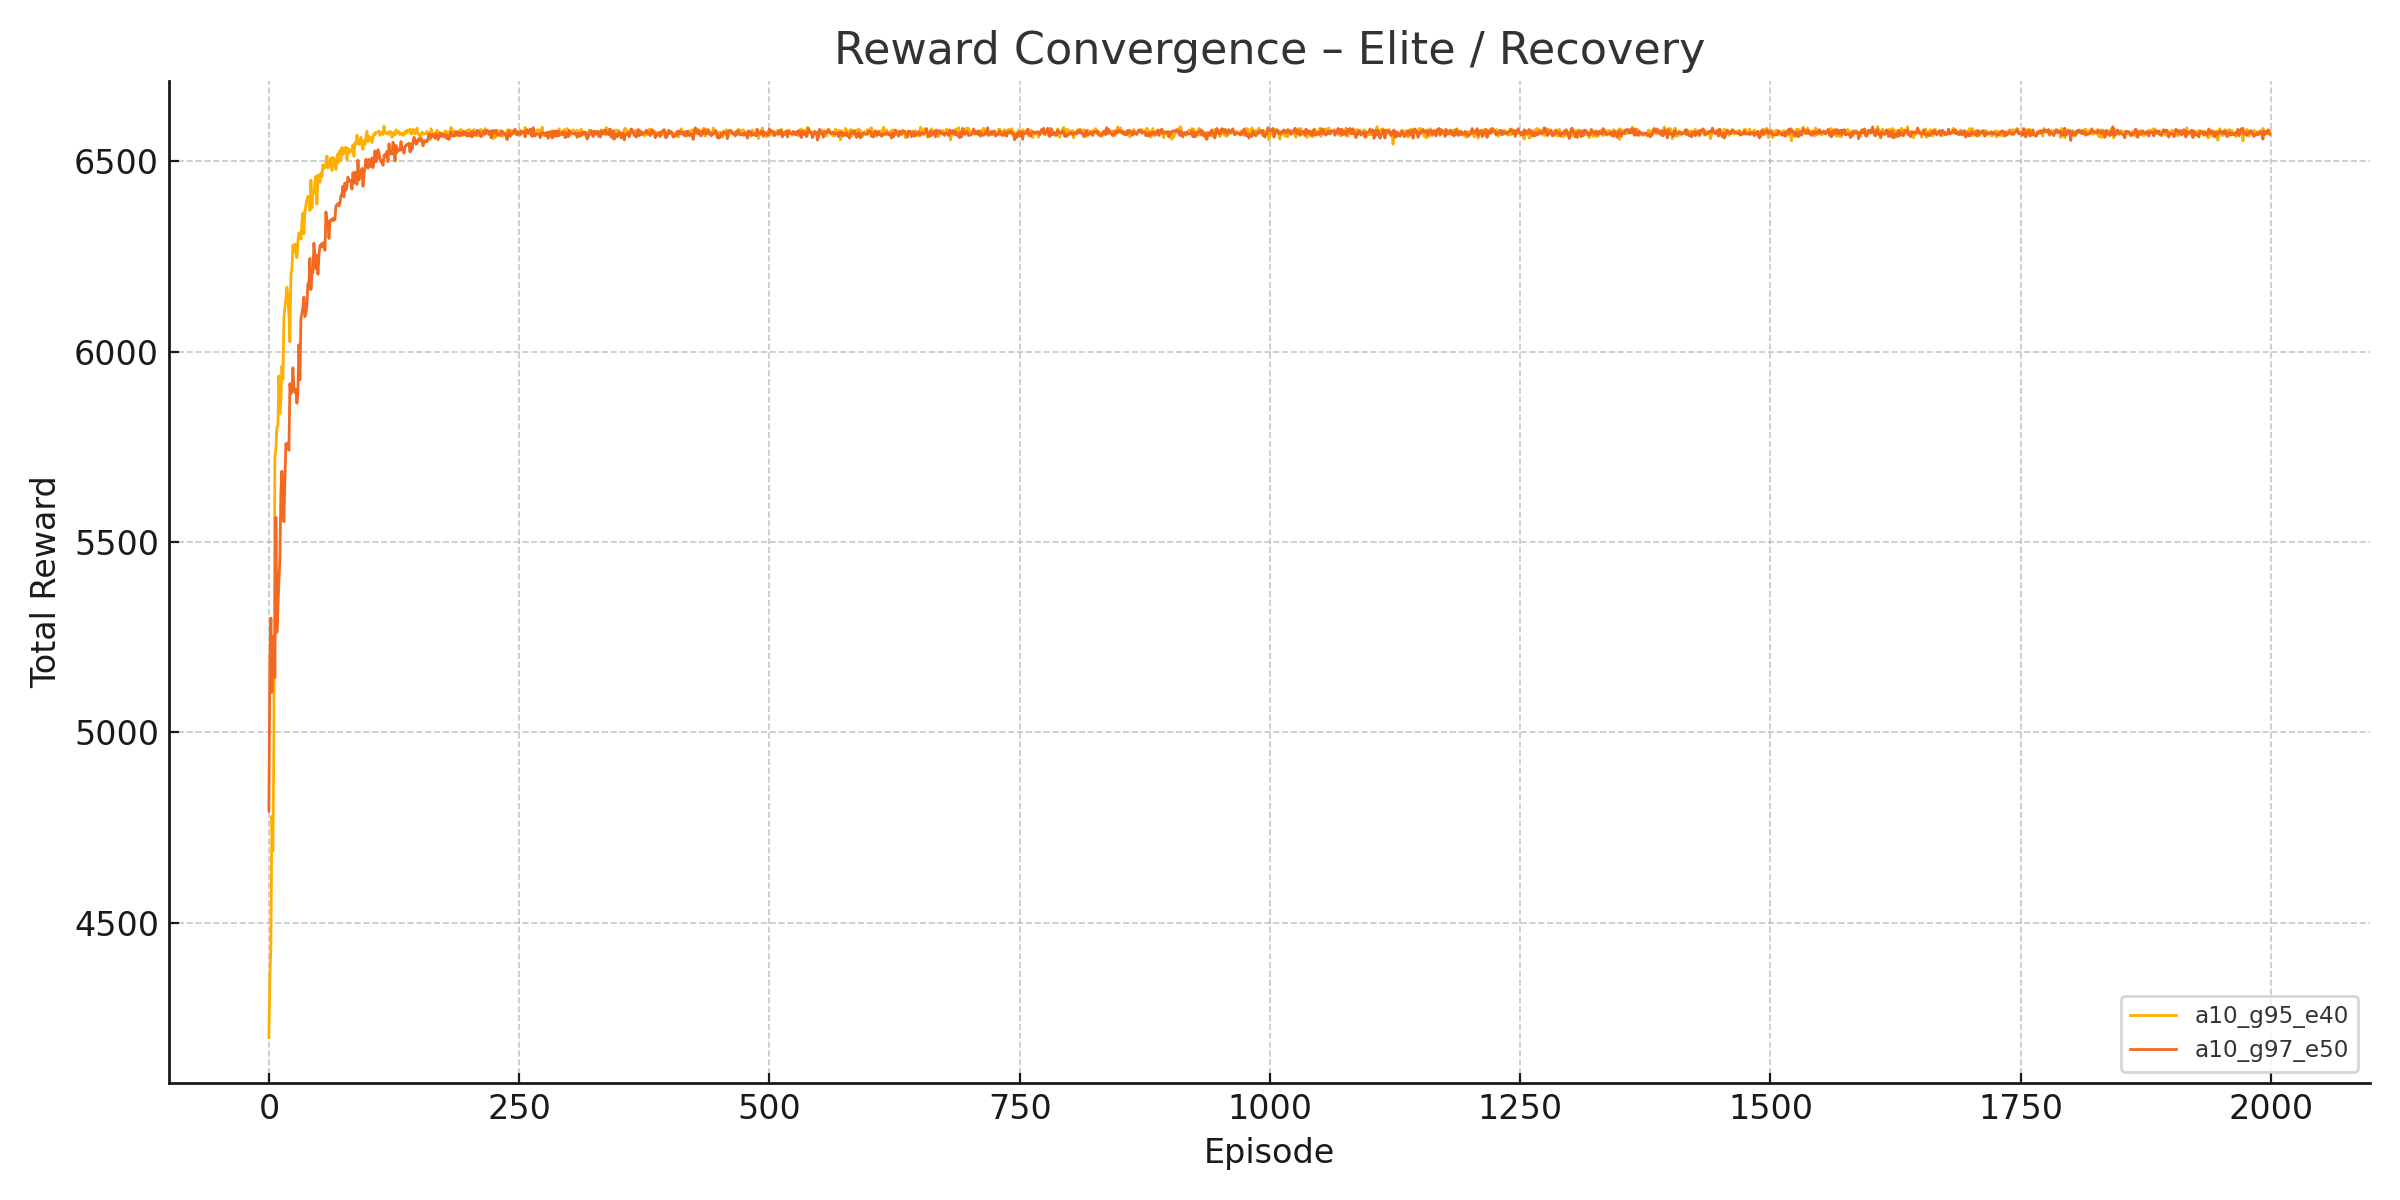
\includegraphics[width=\textwidth]{images/elite_recovery_convergence.png}
    \caption{Recovery}
  \end{subfigure}
  \caption{Reward convergence for \textbf{Elite} (2000 episodes)}
  \label{fig:elite_convergence}
\end{figure}


\begin{figure}[htbp]
  \centering
  \begin{subfigure}[b]{0.45\textwidth}
    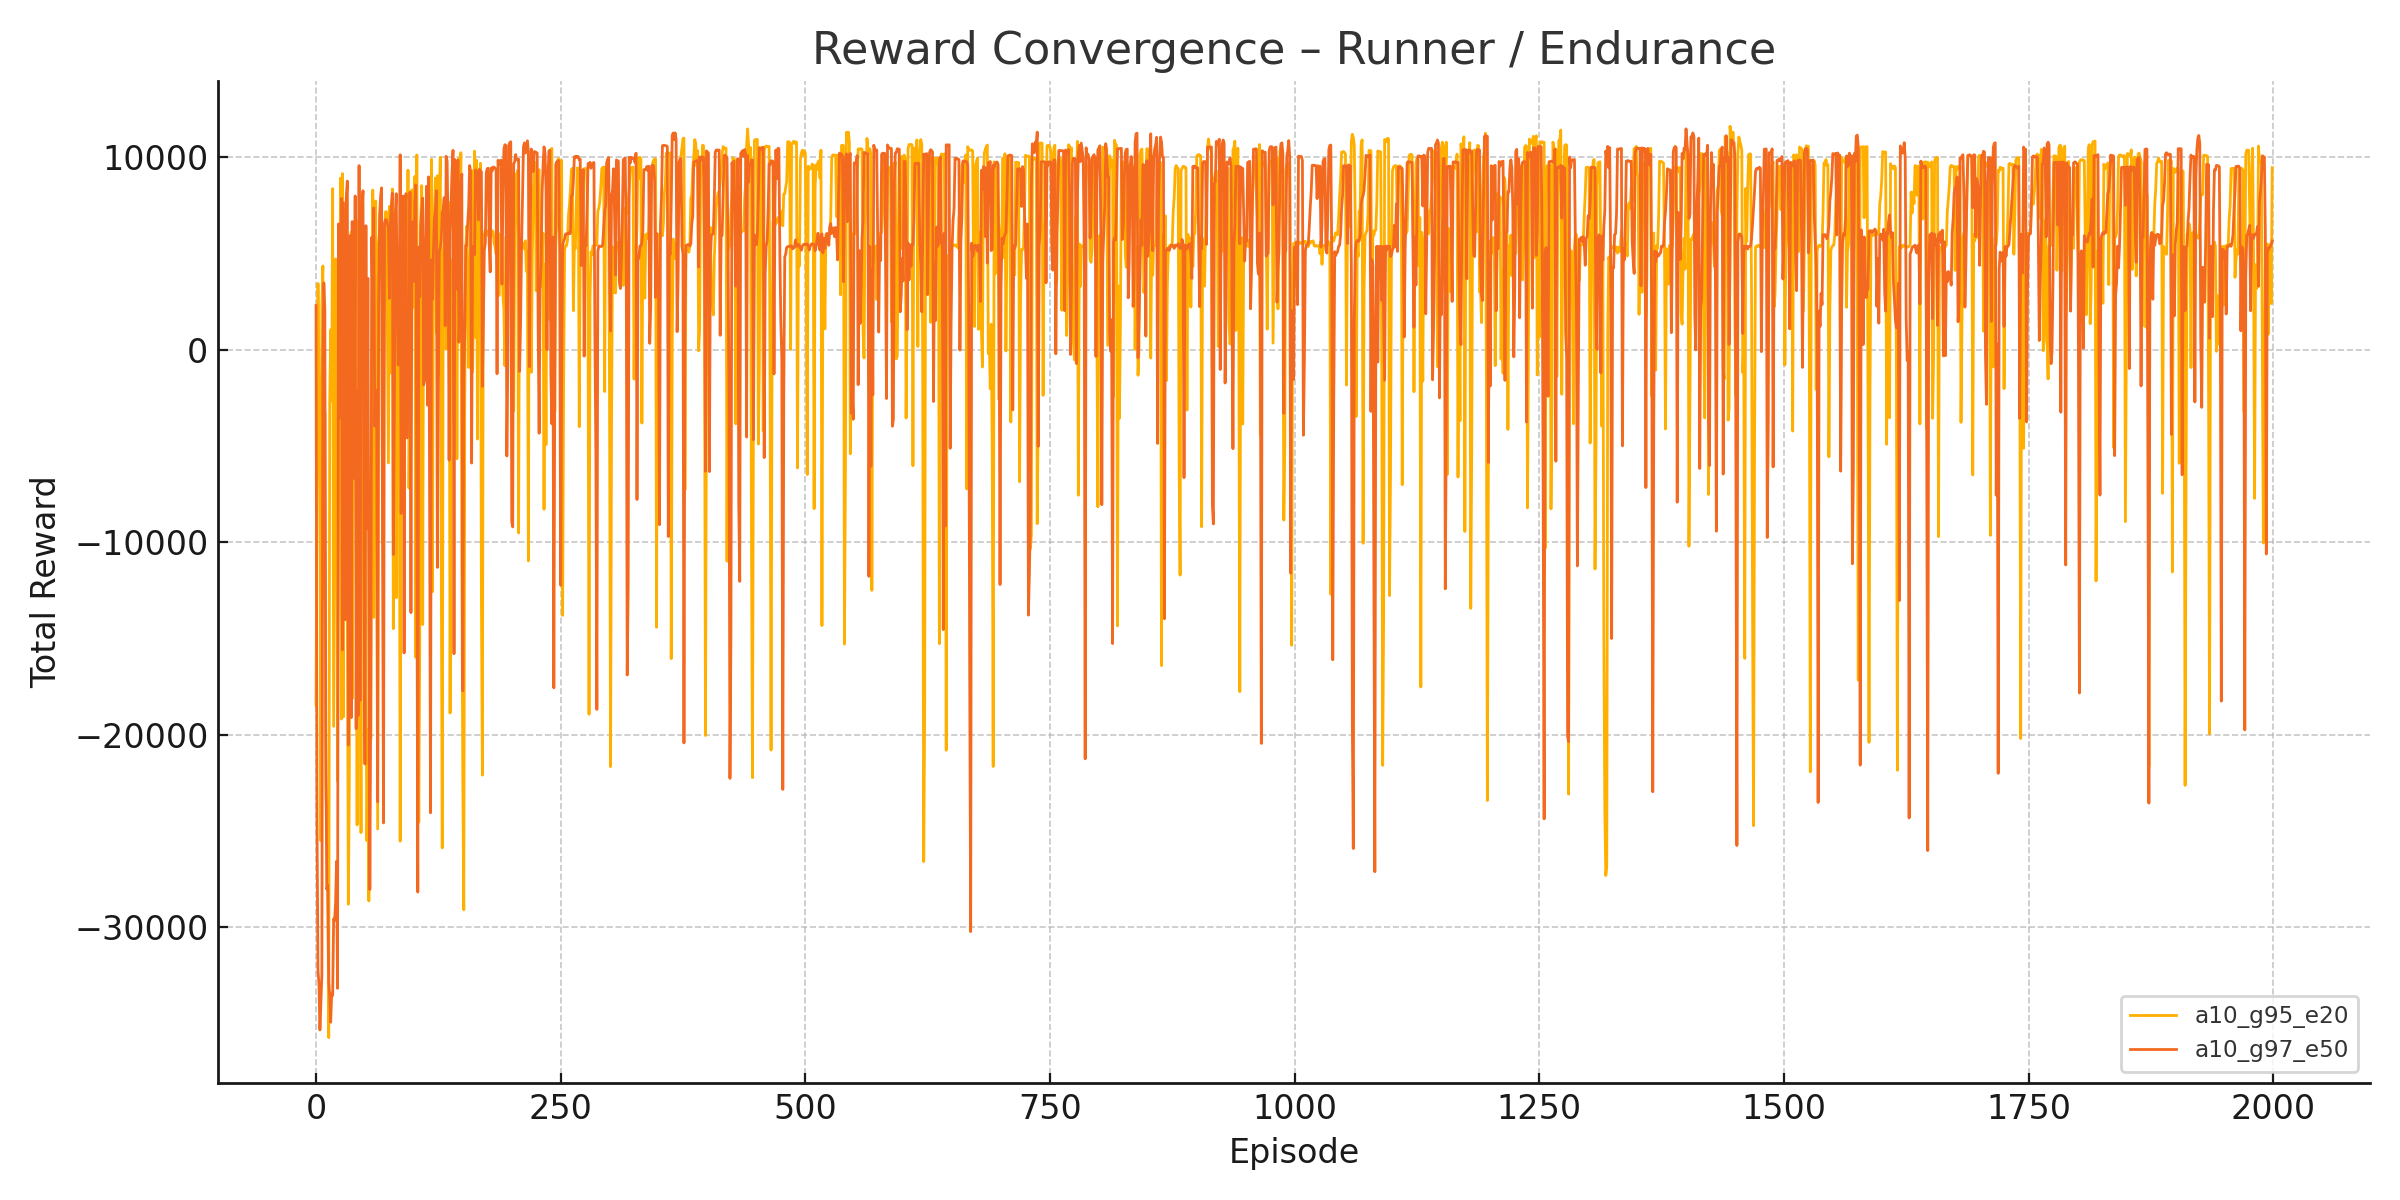
\includegraphics[width=\textwidth]{images/runner_endurance_convergence.png}
    \caption{Endurance}
  \end{subfigure}
  \hfill
  \begin{subfigure}[b]{0.45\textwidth}
    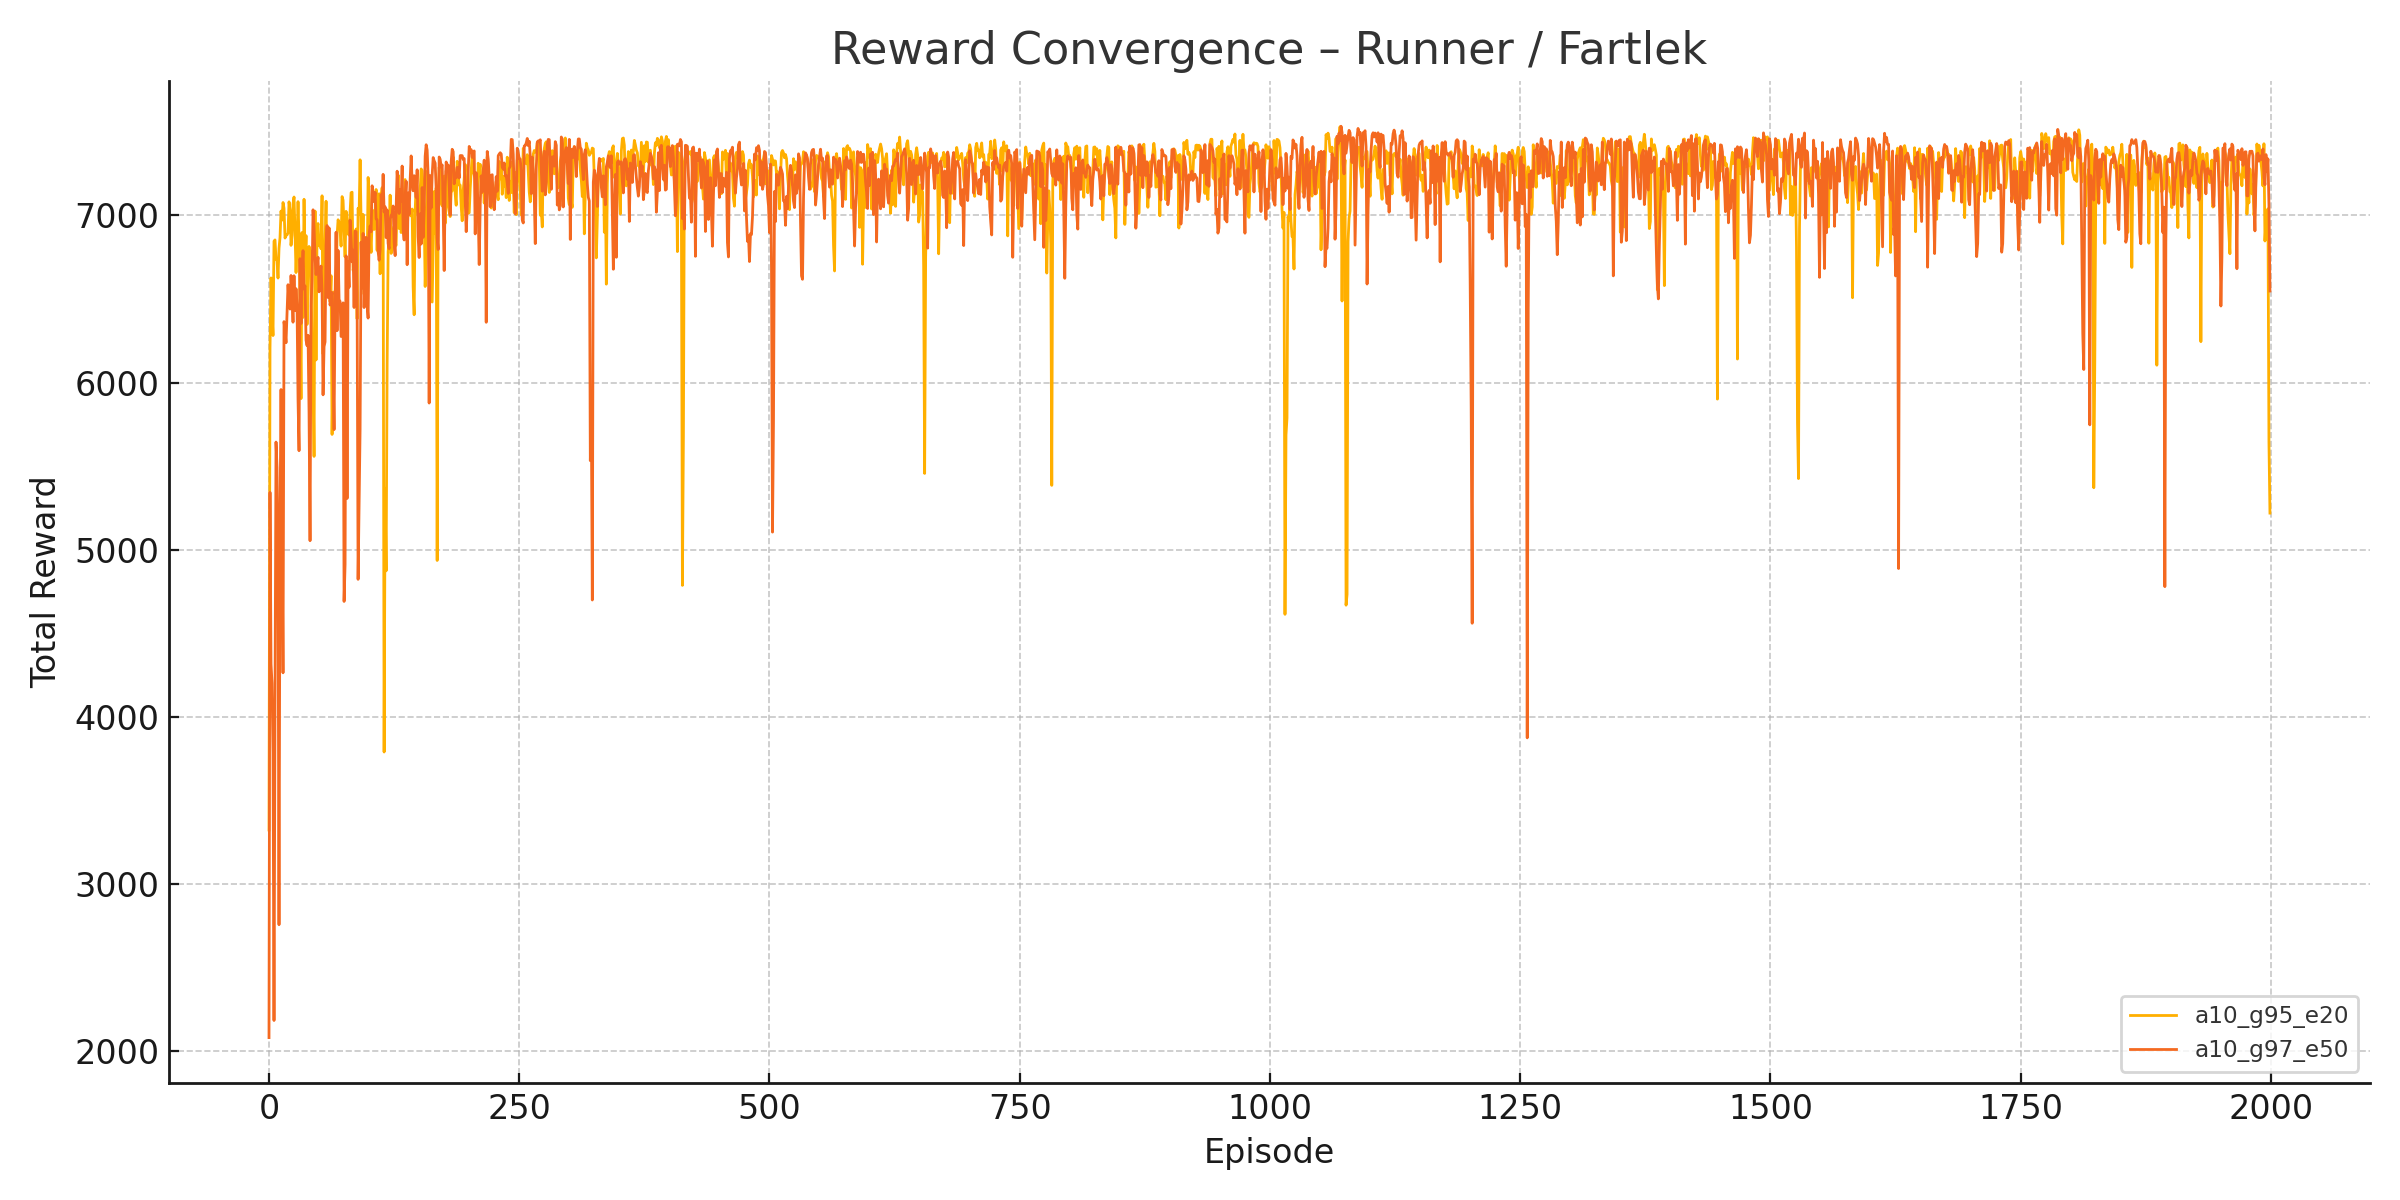
\includegraphics[width=\textwidth]{images/runner_fartlek_convergence.png}
    \caption{Fartlek}
  \end{subfigure}
  \vskip\baselineskip
  \begin{subfigure}[b]{0.45\textwidth}
    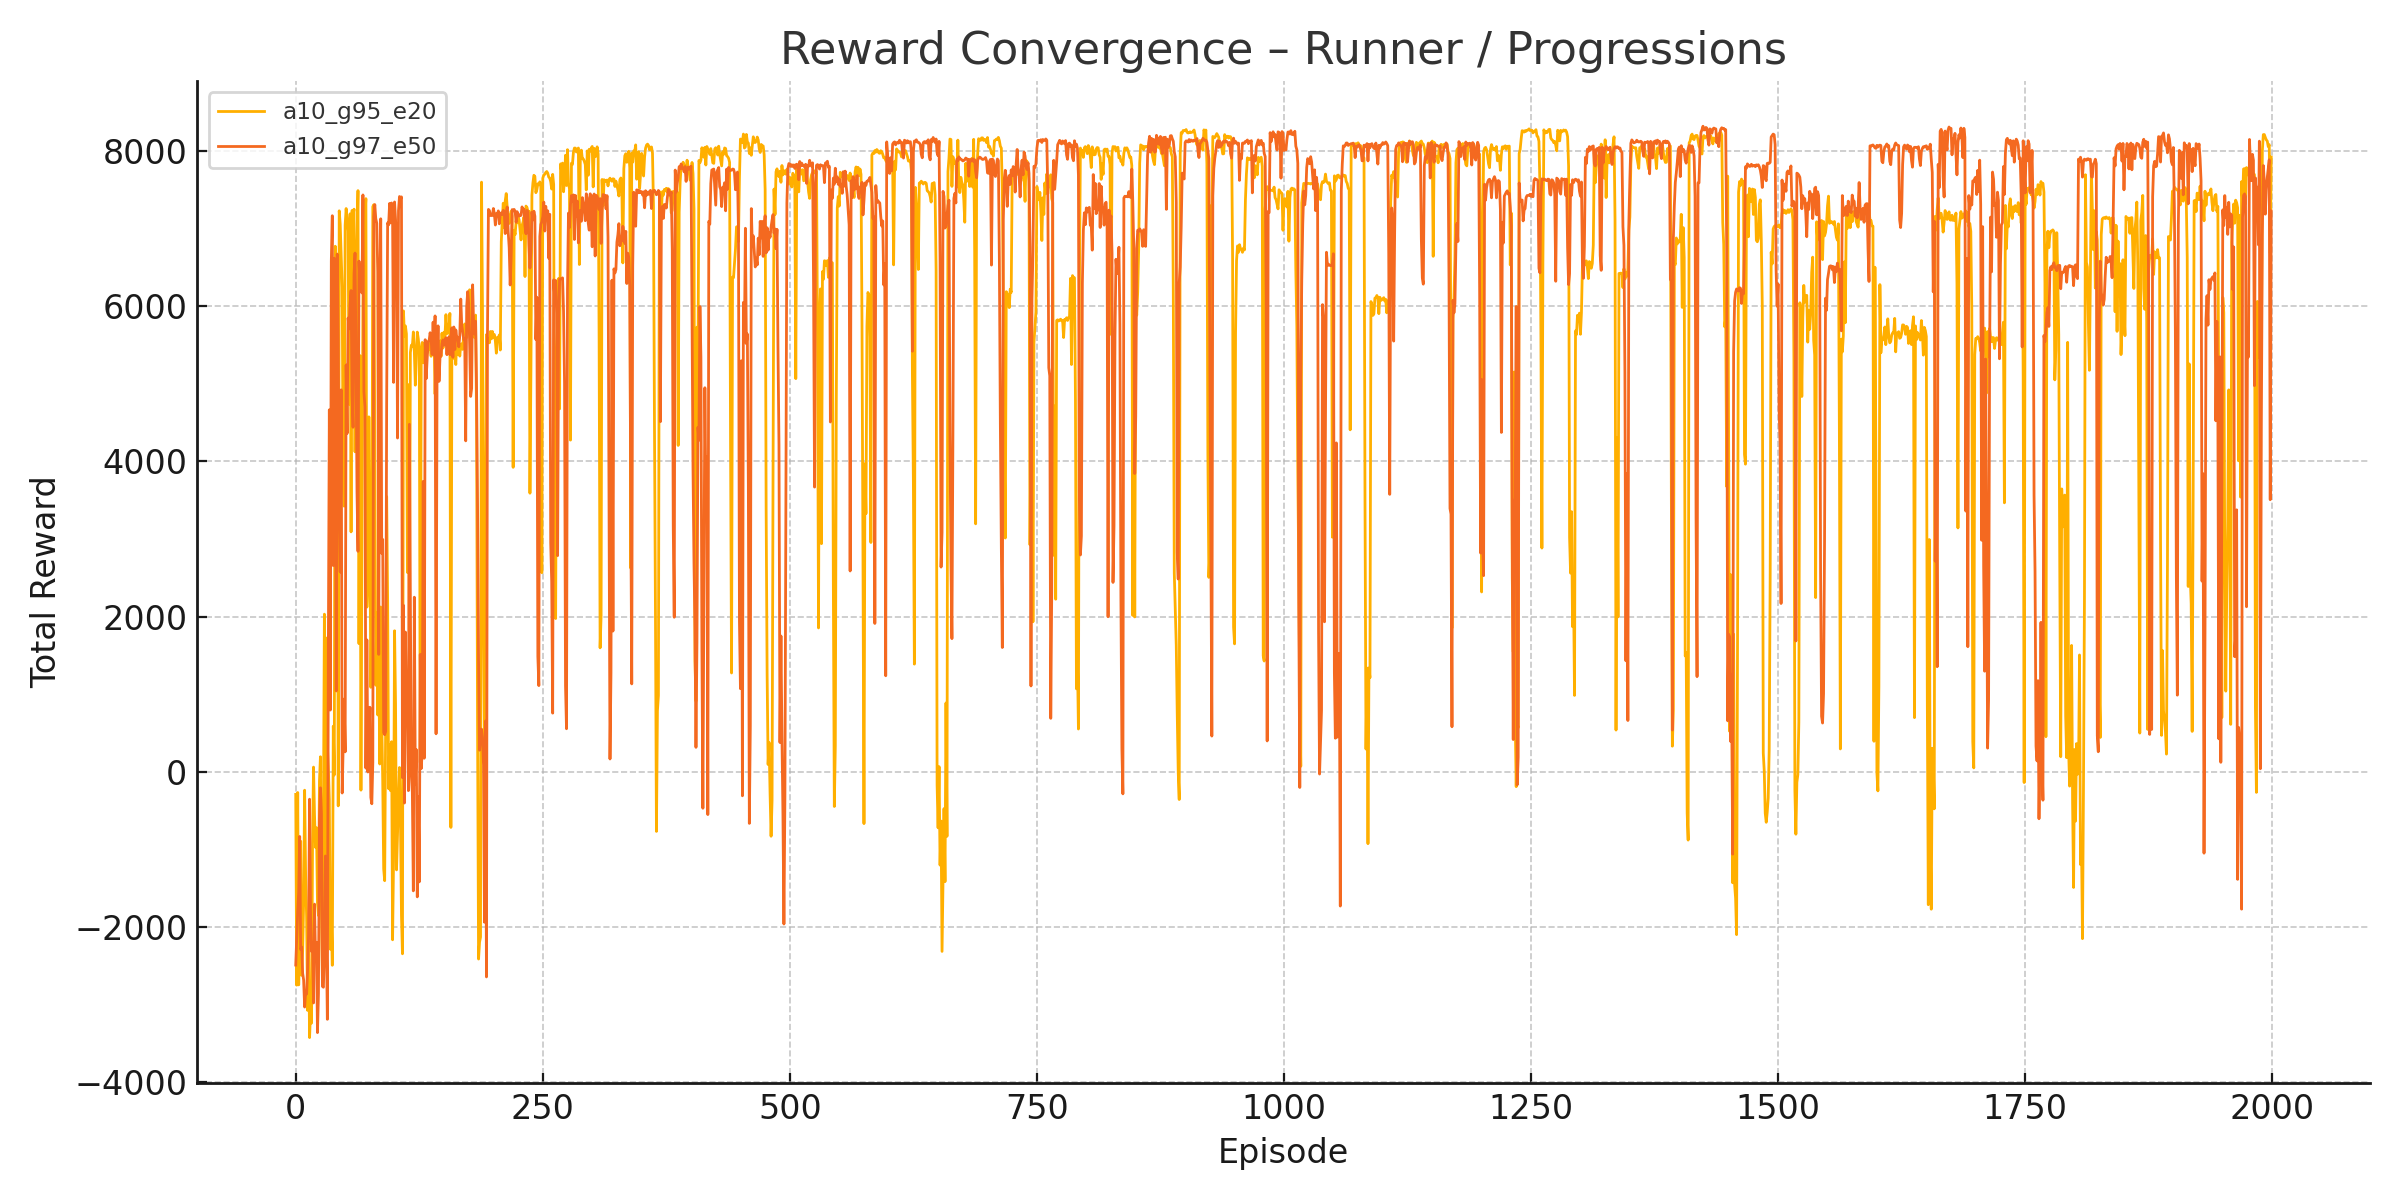
\includegraphics[width=\textwidth]{images/runner_progressions_convergence.png}
    \caption{Progression}
  \end{subfigure}
  \hfill
  \begin{subfigure}[b]{0.45\textwidth}
    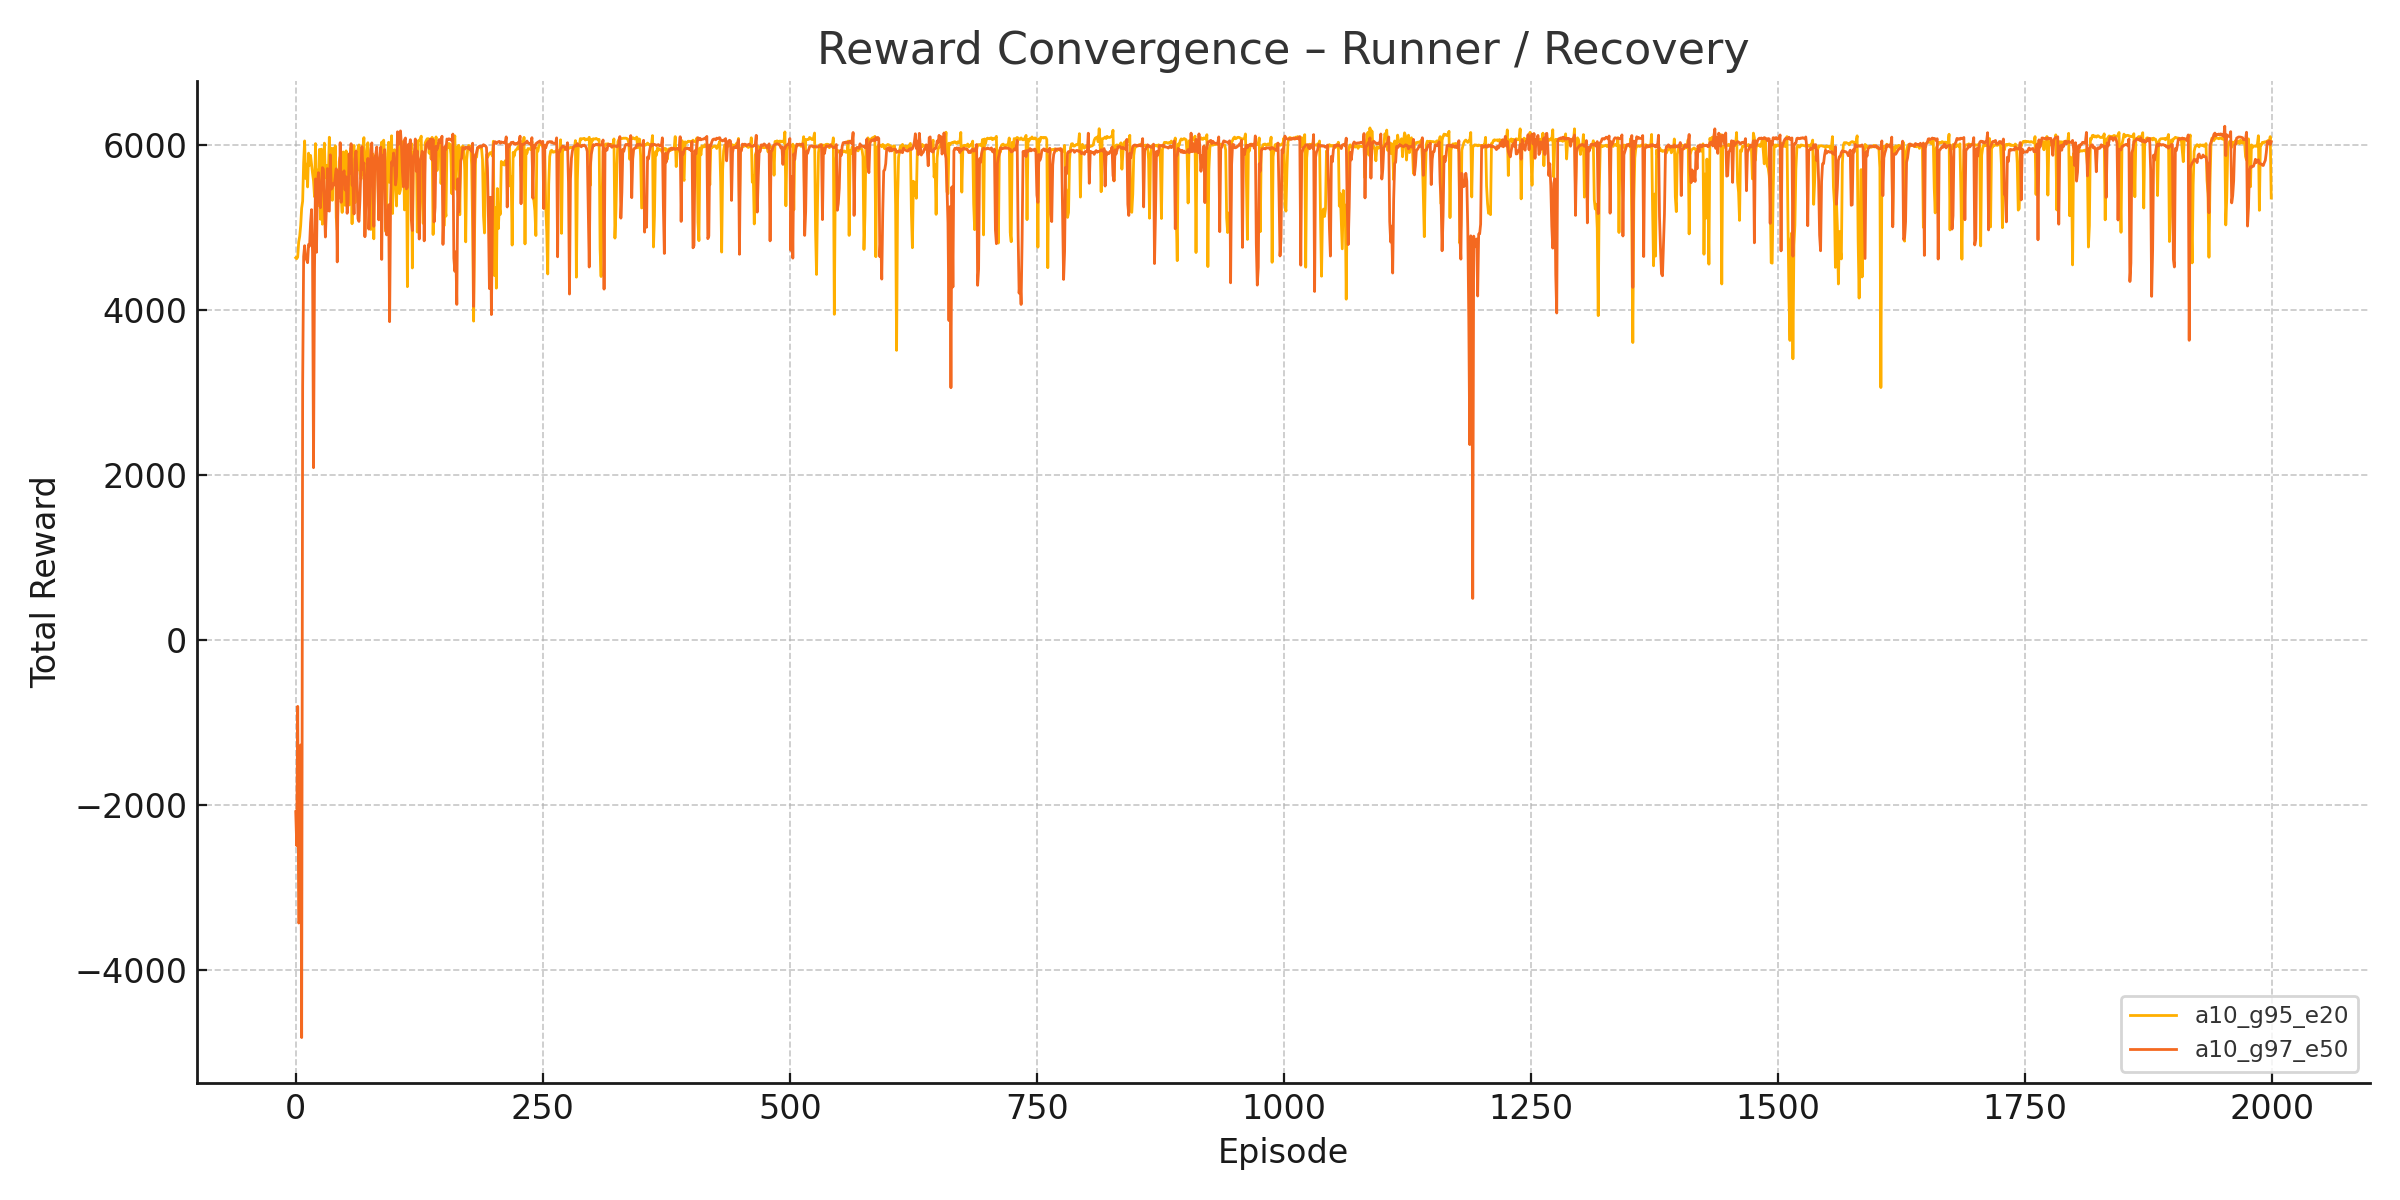
\includegraphics[width=\textwidth]{images/runner_recovery_convergence.png}
    \caption{Recovery}
  \end{subfigure}
  \caption{Reward convergence for \textbf{Runner} (2000 episodes)}
  \label{fig:runner_convergence}
\end{figure}


\begin{figure}[htbp]
  \centering
  \begin{subfigure}[b]{0.45\textwidth}
    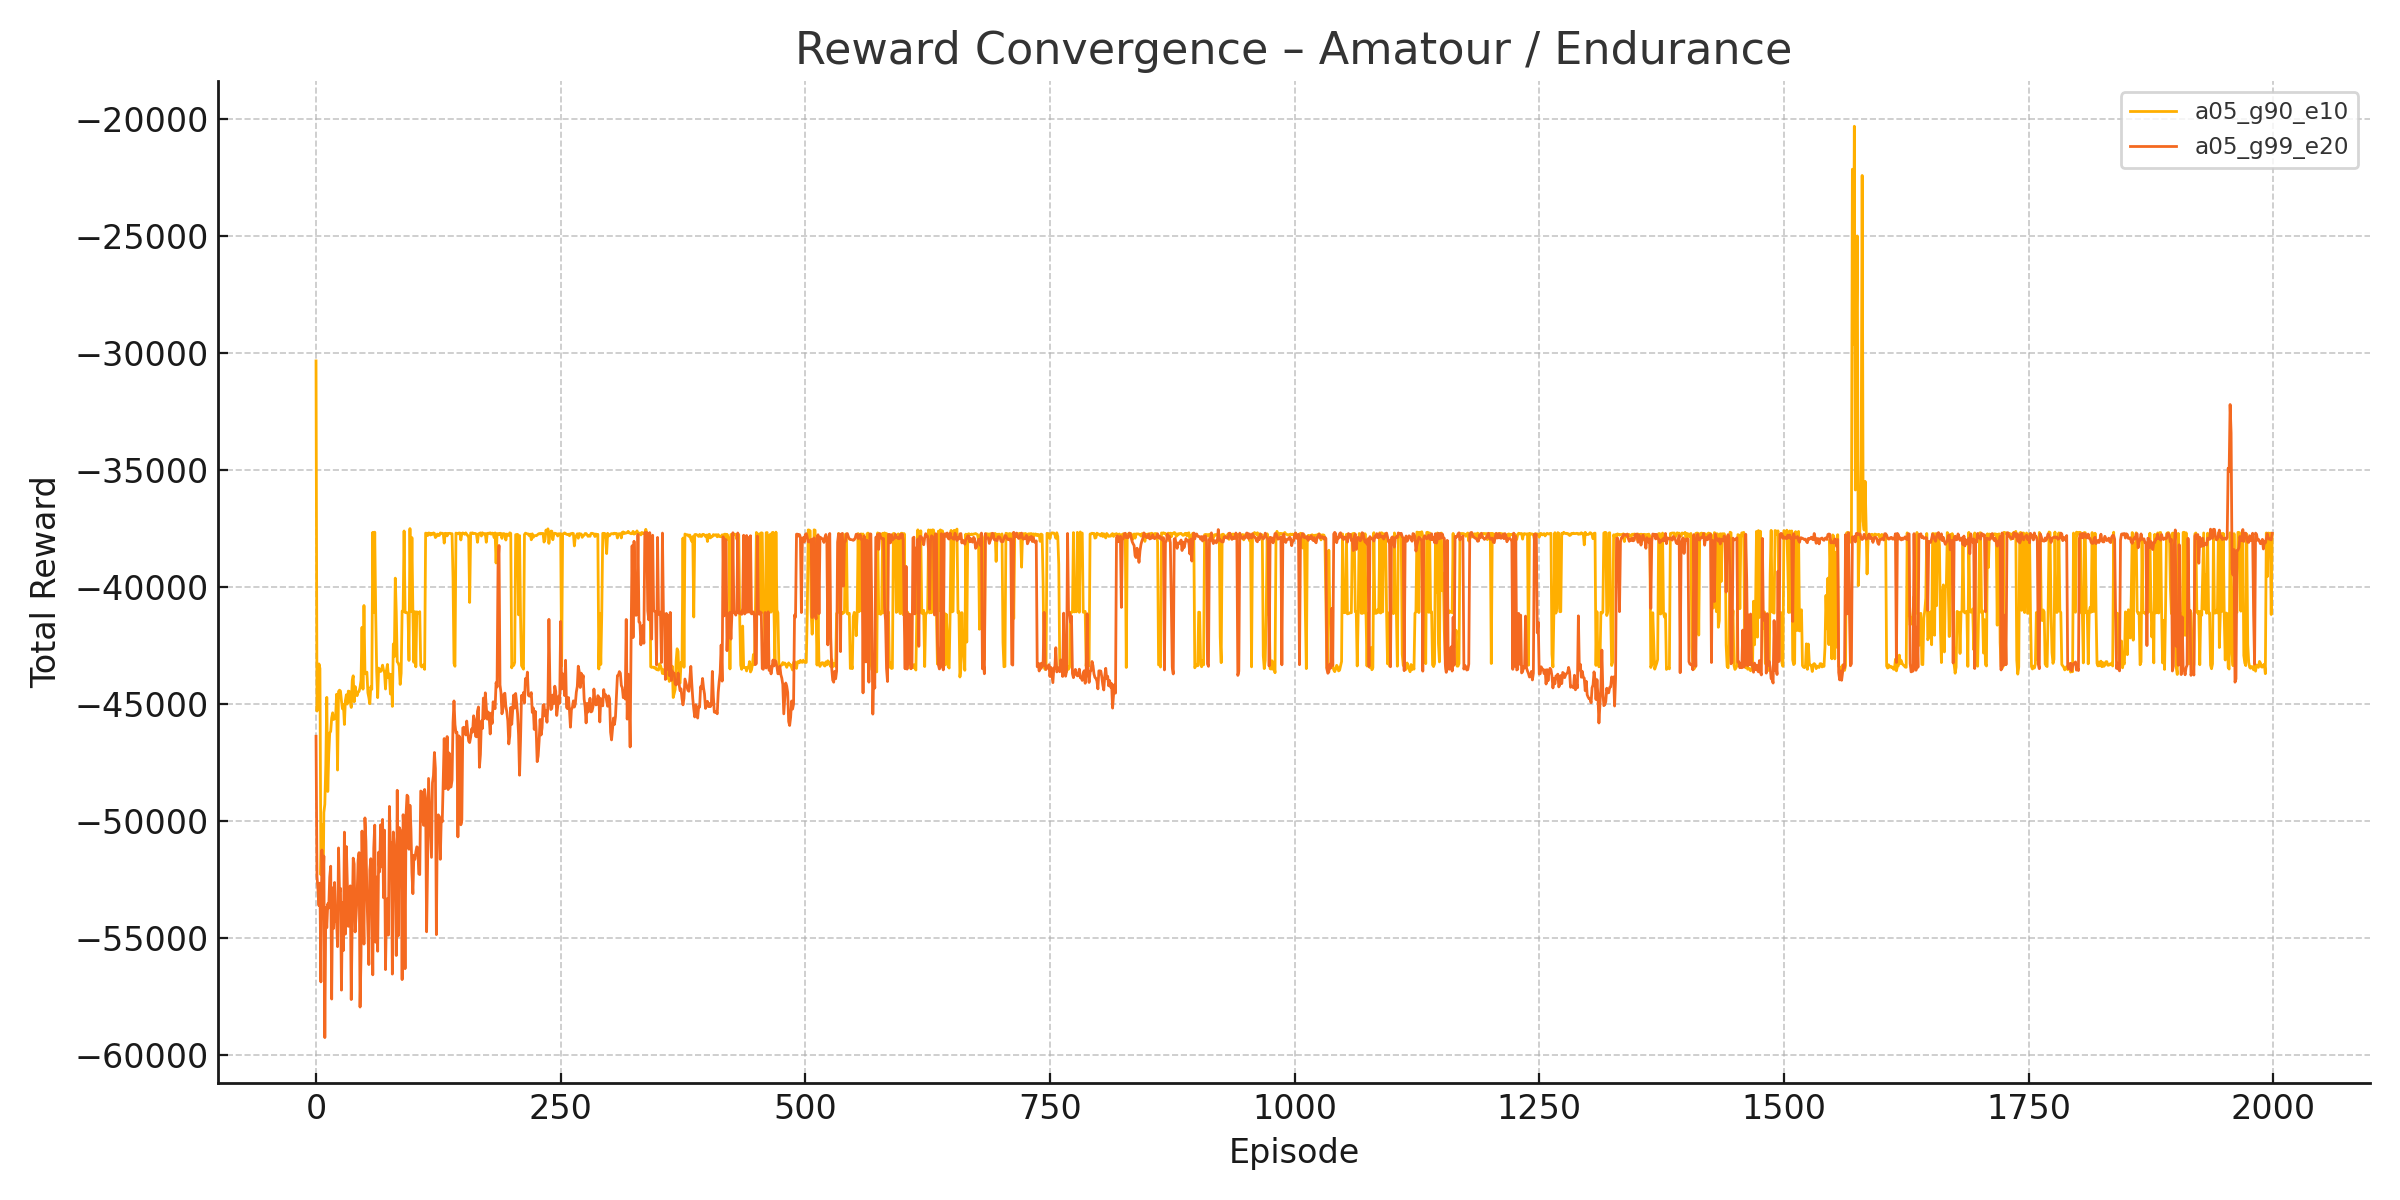
\includegraphics[width=\textwidth]{images/amatour_endurance_convergence.png}
    \caption{Endurance}
  \end{subfigure}
  \hfill
  \begin{subfigure}[b]{0.45\textwidth}
    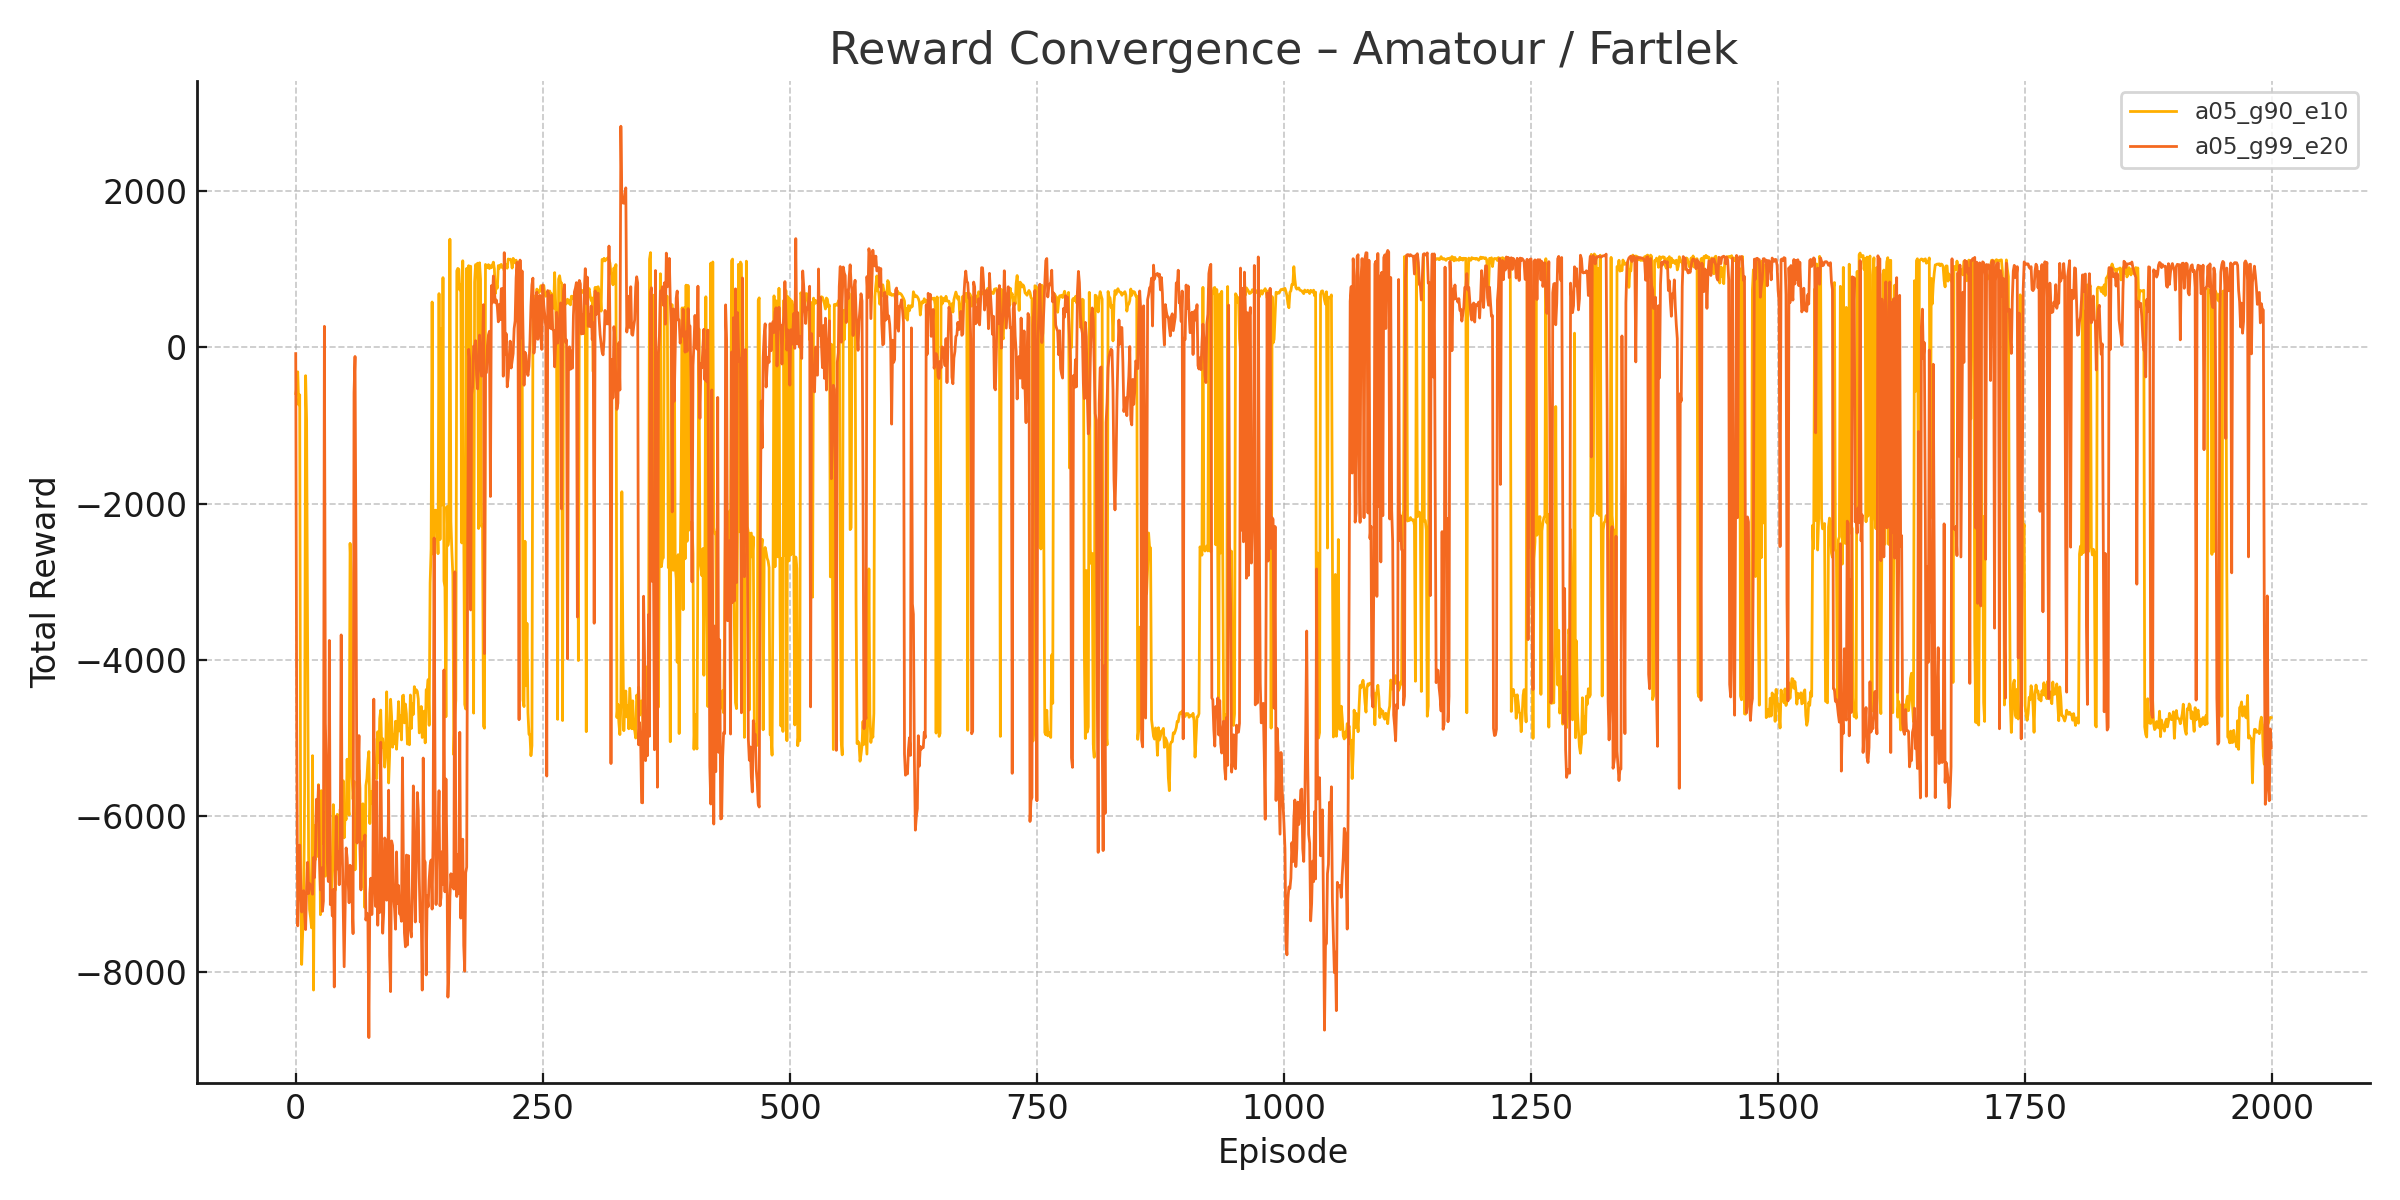
\includegraphics[width=\textwidth]{images/amatour_fartlek_convergence.png}
    \caption{Fartlek}
  \end{subfigure}
  \vskip\baselineskip
  \begin{subfigure}[b]{0.45\textwidth}
    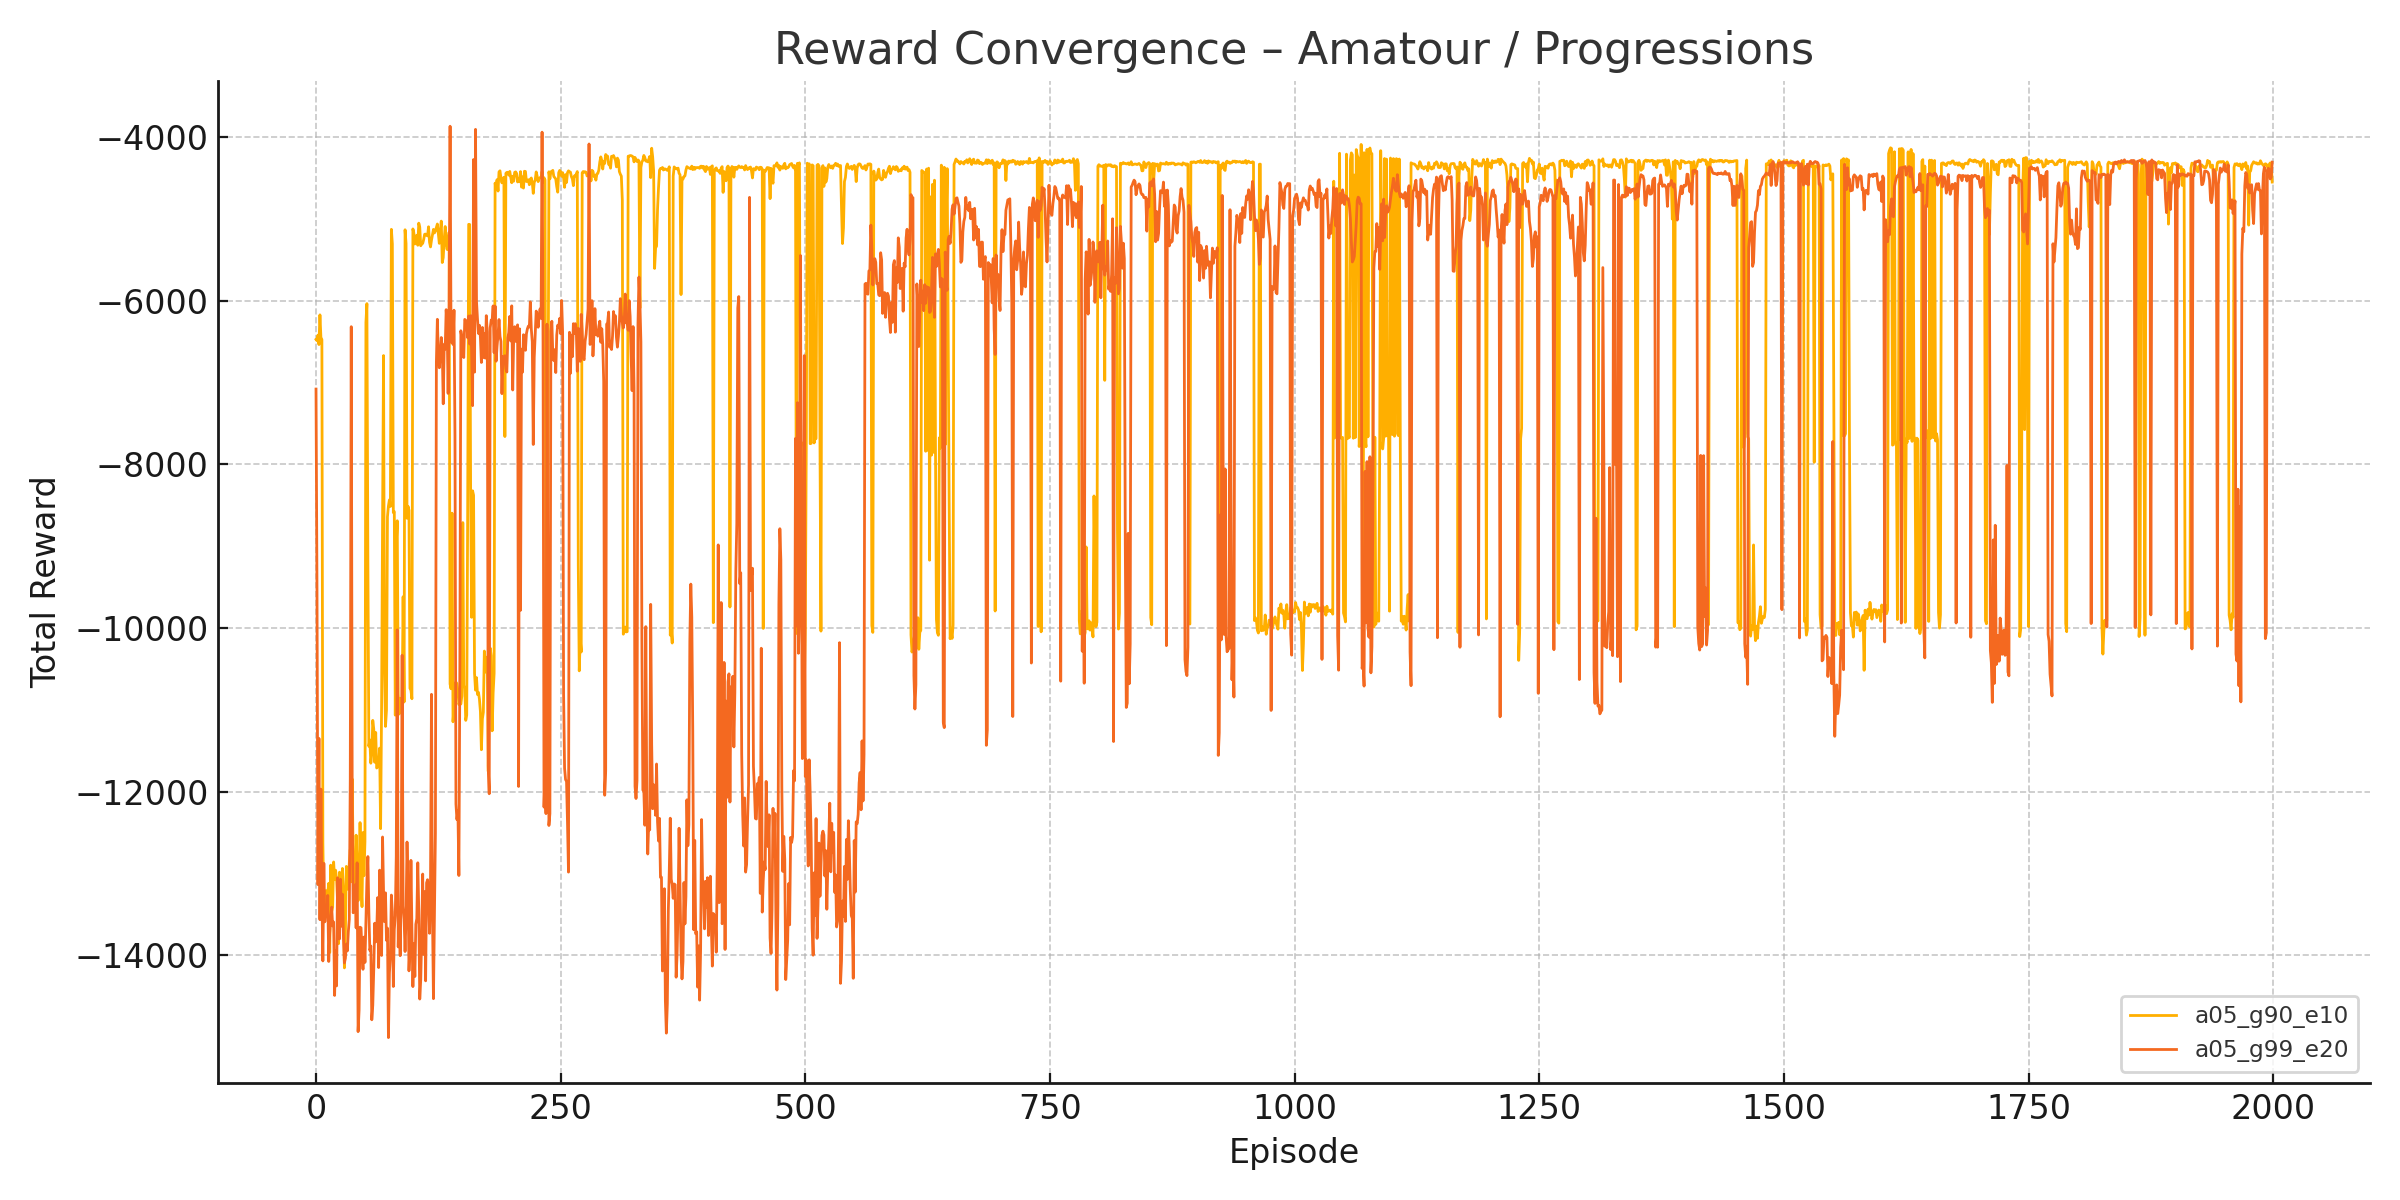
\includegraphics[width=\textwidth]{images/amatour_progressions_convergence.png}
    \caption{Progression}
  \end{subfigure}
  \hfill
  \begin{subfigure}[b]{0.45\textwidth}
    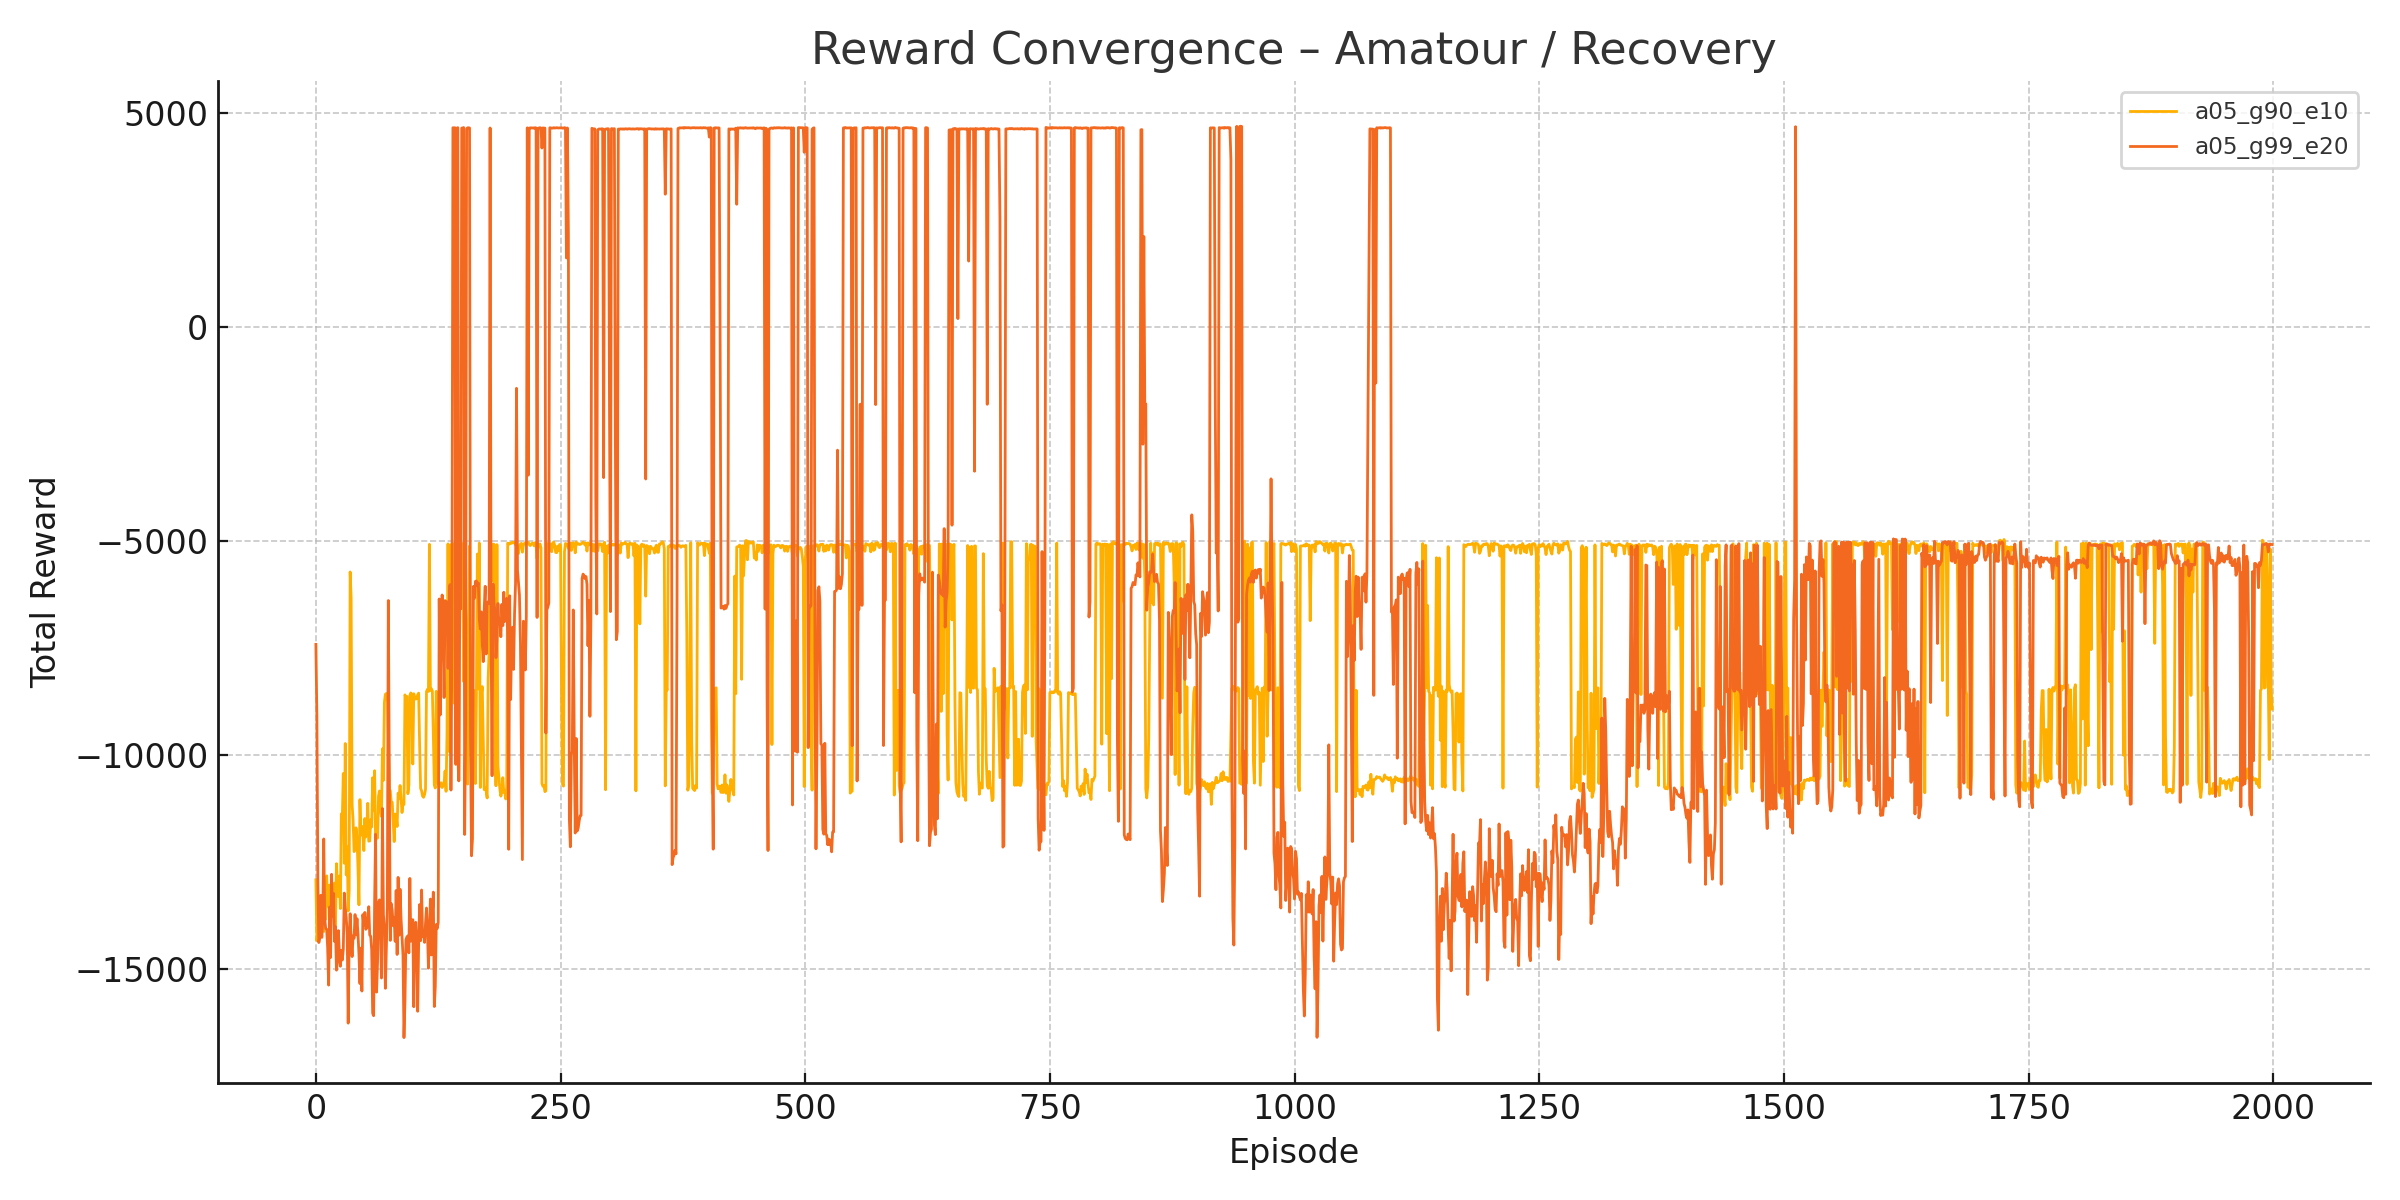
\includegraphics[width=\textwidth]{images/amatour_recovery_convergence.png}
    \caption{Recovery}
  \end{subfigure}
  \caption{Reward convergence for \textbf{amateur} (2000 episodes)}
  \label{fig:amateur_convergence}
\end{figure}


\subsection{Final Decision and Q-table Selection}

The second experiment identified the best hyperparameters for each athlete profile:

\begin{itemize}
    \item \textbf{Elite}:   \texttt{alpha=0.1, gamma=0.97, epsilon=0.5, decay=0.98}
    \item \textbf{Runner}:  \texttt{alpha=0.1, gamma=0.95, epsilon=0.2, decay=0.99}
    \item \textbf{amateur}: \texttt{alpha=0.05, gamma=0.90, epsilon=0.1, decay=0.98}
\end{itemize}


\section{Challenges and Future Developments}\label{sec:challenges-future}
\section{Limitations and Future Improvements}\label{sec:limitations}

\subsection{State-space explosion}
The current Markov model already spans seven discrete variables, yielding several thousand reachable combinations.  Extending realism would require additional factors — e.g.\ \emph{weather} (temperature, humidity, wind) and \emph{surface type} (asphalt, track, trail, grass). Although essential for real-world fidelity, every new dimension inflates the state complexity.

\subsection{Richer athlete profiles}
Present profiles depend on basic informations and a FTP valu. A more faithful description would incorporate sex, age, injury history, recent training load, previous-night sleep quality, HRV-derived recovery indices and update them with the evolution of the training process. 
Such metadata would enable session prescriptions that respect female hormonal cycles, age-related recovery kinetics, and cumulative muscle stress.

\subsection{Fatigue and reward refinement}
Fatigue and reward terms were the hardest features to properly develop. In order to be even more realistic and coherent with real life behaviours could be implemented also a \textbf{Injury-risk term}, which will introduce a weekly load delta component that penalises abrupt increases in training load, reducing overuse-injury likelihood.
Another possibl improvement could be the introduction of \textbf{sleep quality} and \textbf{recovery indices} as additional reward terms, which would allow the agent to adapt its pacing strategy based on the athlete's recovery status. This could be particularly useful for athletes with varying sleep patterns or those recovering from intense training sessions.

\subsection{Temporal resolution}
All decisions are issued at 1 Hz. Increasing the control loop to 5–10 Hz — or adopting event-driven updates triggered by rapid HR changes would shorten feedback latency and smooth the athlete's perceived guidance.

\subsection{Personalised on-line learning}
After the first ten sessions, enough data exist to characterise an individual pacing style.  Fine-tuning the policy with a small neural network head (e.g.\ policy-gradient or Soft Actor Critic) on top of the pre-trained Q-table would capture personal patterns without restarting from scratch.  
Meta-learning techniques could further shrink the cold-start phase for new athletes.


\bigskip
Addressing the above points will increase both realism, athlete safety but most importantly will move \emph{Smart Pacer} closer to a deployable digital coach that can adapt to individual needs and conditions, providing a more effective and personalized training experience.

\end{document}
